%!TEX root=../tax-democracy-held.tex

\chapter[Hypotheticals Matter]{Why Hypotheticals Matter} \label{chap:hypotheticals-matter}

%\section{Anthrodicy} \label{sec:Anthrodicy}

%\begin{quote}
%	\emph{``It is demonstrable'' said he,``that things cannot be otherwise than they are; for as all things have been created for some end, they must necessarily be created for the best end. %Observe, for instance, the nose is formed for spectacles; therefore we wear spectacles. The legs are visibly designed for stockings; accordingly we wear stockings. Stones were made to be hewn and to construct castles; therefore my lord has a magnificent castle; for the greatest baron in the province ought to be the best lodged. Swine were intended to be eaten; therefore we eat pork all year round. And they who assert that everything is right, do not express themselves correctly; they should say that everything is best.
%	''}\\*
%	--- Dr.~Pangloss in Voltaire's novella \emph{Candide} (\citeyear{Voltaire1759}: K125).
%\end{quote}
%
%
%\begin{quote}
%	\emph{``When the general atmosphere is bad, language must suffer. I should expect to find --- this is a guess which I have not sufficient knowledge to verify --- that the German, Russian and Italian languages have all deteriorated in the last ten or fifteen years, as a result of dictatorship. But if thought corrupts language, language can also corrupt thought. A bad usage can spread by tradition and imitation even among people who should and do know better.''}\\*
%	--- \cite{Orwell1946}
%\end{quote}
%
%\begin{quote}
%	\emph{``We've got a bad thing made by men, and by God, that's something we can change.''}\\
%	--- Anonymous tenant in \emph{The Grapes of Wrath} \citep[38]{Steinbeck1939}
%\end{quote}
%
%So \emph{really}, is all ``for [\ldots] the best [\ldots] in the best of all possible, [liberal-democratic, capitalist] worlds''  (\emph{ibid.}: K428ff).
%
%Today, Dr.~Pangloss, the 18th century teacher, might feel vindicated in this Leibnizian \citeyearpar{Leibniz1710} optimism. Since industrialization set on in his age, the developed economies have grown annually by initially 1.3\%, then 3.1\% in GDP per capita (\citealt{Easterlin2000}: 10f), prospering as no human society ever has \citep{DeLong1998}. Since enlightenment dawned at his time, the established democracies have fostered peaceful mass participation and liberal democracy continues to proliferate \citep{Huntington-1991-aa}.
%
%But Candide, Voltaire's hapless title character and Pangloss' na\"{i}ve student, might still stumble into misfortune, and despair over the hardship of (some) contemporary lives. In the richest of countries, he might be dismayed by growing poverty (for example, \citealt{Bundesregierung2006} for Germany, widening inequalities of wealth and income (for example, \citealt{Grabka2007a}: 138 for Germany, \citealt{Bucks2006} for the US), crumbling public services and state budgets in crisis or default. In the richest of times, he might be troubled by the dark shadows of global warming (for example, \citealt{Stern-2006-aa}), aging populations (for example, \citealt{Demeny-2003-aa}: 2, \citealt{Borsch-Supan2000}) and stalled productivity %add source
%looming over our long-term prosperity. \marginpar{Include other, OECD-wide sources.} In the oldest of republics, he might be repelled by distorted debates and decision-making deadlocked %add source,
%and in the finest of democracies, he might be frustrated by ill-informed \citep{Delli-CarpiniKeeter-1996-aa}, ignorant, %add citation
%irrational \citep{Caplan2007} and dissatisfied voters \citep{PutnamPharr-2000-aa}.
%
%Candide's puzzled lament, in the novella as in the real world, does not lead anywhere. He does not specify what would mark a better world, does not consider what limits may govern the real world, and suggests no path to progress. Such discontent without alternative is impotent.
%
%But Pangloss' unwavering affirmation of the status quo does not lead us anywhere either. He, the (satirized) learned scholar, does not so much``admirably prove[\ldots] that there is no effect without a cause'' (\citealt{Voltaire1759}: K36) but mindlessly naturalizes the existing state of affairs. He disavows alternative or even better worlds and thereby fails to explain the cause for their non-effect and betrays the humanist calling of science. Such analysis without alternative is fallacious and amoral.

%Genschel 200 deutscher Artikel
	%Both the sceptics and apologetics of the race to the bottom are wrong.
	%There is indeed no empirical evidence for a race to the bottom \ldots
	%\ldots but that is not because of no competition, but because there is at the same time a need for greater state spending and the inability to tax other things (labor, consumption, indirectly) without doing great harm
	%results are: labor and consumption don't flee the country, but you get unemployment and a shadow economy.
	%the above is all p 268
	%I think it is wrong to assume great unemployment to be "given", it is rather caused by the inability of the state to tax other stuff.
	%Genschel 2000 269 points out that present tax regimes are historical artefacts, from a time of closed borders.
	%two assumptions overall: taxation would decrease, but also: relocate to less mobile things (labor, consumptioN)
	%Genschel finds: total tax stayed the same, but expenditures grew faster than revenue, hence public debt
	%There is a fundamental problem with Genschel's argument. Körperschaftsteuer ? corporate tax doesn't necessarily tax capital. It depends. Wealth taxes have in fact, decrased (!).
	%Genschel's analysis oif tax revenue is superficial. It does not disaggregate capital, labor, stock and flow taxation.also, as Genschel concedes, the share of taxes in revenue does not tell us anying about how  redistribute it really still is.
	%look at EUROSTAT implicit tax rates
	%Genschel does mention ibid 274, that in fact, it is likely that there was some tax competition, and that it lead to fewer tax increases overall, particularly on capital.
	%Genschel cites examples ibid 285 how progressivity was reduced to avoid tax flight - it's simple, the transaction costs for fleeing are relatively lower. Yet there is no normative justification to not tax capital income progressively.
	%Umsteuerung auf Verbrauchssteuern (Genschel 288) is bullshit, because they are just as regressive. and also: procyclical, hits labor intensive service industry, with high price sensibility in particular (you won't go to the restaurant)
	%Please mention that taxing capital, in and of itself, is also problematic in welfare terms. It's not the perfect tax, because we want capital accumulation.
	%Mention Genschel's treatment of intelligent tax-evasion through intra-company strategies.
	%Genschel 1999 is hopeful about ways to resolve the prisoners' dilemma.
	%repeated games, shadow of the future
	%institutions
	%transparency, monitoring
	%but again, they say: it may not be a defection problem, but zero-sum distribution between small and large states
	%my bottom line: empirical pictures are always messy, complicated. But still, if you introduce a normative hypothetical, it is obvious that really, the situation is quite dramatic.
	%Genschel calculates how large the coalition would have to be (421)! his is awesome!
	%note later comparison to trade union theory and trade creation vs.\ trade diversion

%Gesnchel 2005
	%53 brilliantly right: "The effect (of globalization) is not so much to force change upon the tax state as to reduce its freedom to change"
	%Schumpeter indeed: "the revenue of the state is the state" (53
	%genschel 60 also points to the problem of multinationals: where to tax them and on what?!?
	%make a bigger argument about why taxing corporations is a bad idea: they are not natural persons, they don't need to be progressive or can they. The story of tax evasion and tax avoidance, frequently with firms with no people in off-shore havens goes to show the futility of this exercise: on which fundamental basis is a firm supposed to be taxed? location? of what? As Genschel puts in the Glaxo (marketing vs.\ R+D argument) argument "It also implies that any national claim to a particular share of Glaxo's profits is hard to justify on the basis of principle." (61 genschel 2005). Expand this argument to the issue of progression.

%from jachtenfuchs paper
			%The summarizing nature of this paper notwithstanding, some critical remarks on the challenges of economic denationalization and the welfare state are made in the following.

		%First, relatively straightforward methodological problems question the validity of the empirical evidence cited by the optimists, particularly by Duane Swank (2005). Welfare regimes are institutions for redistribution and risk-pooling. To investigate the impact of globalization on welfare regimes, it is then necessary to measure to which degree welfare states are still able to fulfill these functions, particularly redistribution. Swank, however, looks at income replacement and others at spending. Obviously and at minimum, public debt and deficits would have to be included in the analysis to warrant the conclusions drawn from the evidence. In the short run, welfare states can – and under political pressure likely will – maintain high benefits even in the absence of sufficient revenues by postponing these costs to future generation. Economic denationalization may reduce the ability of a state to tax and redistribute, not to (over)spend, at least in the short run and under sound monetary policy.

		%More fundamentally, the causal rejection (!) of welfare entrenchment through globalization as put forward by the optimists needs careful positivist research design.  Again minimally, this would require a hypothetical, namely a sufficiently large, prosperous and closed economy. This does not exist in the OECD world, and may not exist at all in reality, as there is a well acknowledged trade-off between liberalization and prosperity. This real world constraint notwithstanding, empirical arguments have to take this methodological problem into account to answer the question whether welfare states can sustainably continue to operate under international economic liberalization.

		%Secondly, the simpler empirical support cited by optimists, including Swank takes a reductionist, inaccurate perspective on globalization as causing capital flight. The economic dynamics of international liberalization are more complicated than that. For instance, the changing relative factor incomes in developed economies in favor of capital, challenge conservative welfare regimes based on taxing labor income and may exacerbate capital accumulation, and, by definition, social inequality (cf.~Stolper-Samuelson theorem, for example in Krugman & Obstfeld 2006). Economic models considering qualification of labor (high skill vs.\ low skill) lead to similar implications, where in developed countries relative labor incomes shift in favor of high skilled people, which, effective labor price floors (through minimum wages or high reservation wages) can lead to economic disequilibrium and structural unemployment.

		%A comprehensive review of the economic implications of globalization is beyond the scope of this critique and certainly beyond my qualification. It should also not be forgotten that liberalization by many models and in many cases is found to be welfare enhancing. But even from a lay-economist’s view, it seems possible, if not likely, that the increased welfare of a globalized economy need not be distributed equitably, in the simplest terms. Rather than simply “capital flight”, an investigation of globalization and welfare entrenchment would have to address issues of possibly diverging factor returns and policy imperatives that result from economic disequilibrium, such as heavy spending on education.

		%Thirdly, lastly, and most fundamentally, the optimists seem to be not so much optimistic about what a welfare state can do, as they seem to be minimal about what it should do. In part, this neoliberal bias follows from an epistemological concentration on the status quo. The research question that Swank, for example answers, is not whether globalization challenges the welfare state. Instead, she argues that it may not affect the status quo of income replacement. This is an unexplicated, negative and minimal definition of the welfare. It assumes that the legislator’s social agenda is limited to income replacement, without regard to broader redistributive issues, particularly the question of who should bear the costs of income replacement. More generally put, this amounts to what the public management literature calls an output perspective on how much money is spend on welfare, in this case.

		%Even to consider anti-discrimination policy, however extensively defined, as an instance of social policy proper, as Leibfried (2005) does, shows the inherent neoliberal bias of this argument. Anti-discrimination, already by name, is negatively defined, and diminishes social policy to be concerned with the abolition of negative constraints, of things we cannot do, of market distortions and at the same time clouds a positive definition of social policy as furthering or freedom to do something, not freedom from something.

		%Welfare regimes are, as Esping-Andersen (1990) has said, systems of stratification in itself, and they have been, from the very beginning socialist demands in the 19th century more than epiphenomenal income replacement. They are tools to socialize the costs of painful, but welfare-enhancing Schumpeterian economic transformations as well as individual hardship and serve as engines to redistribute this very welfare as the legislator wishes. The indeed quintessential and highly political question for globalization and welfare entrenchment is then, whether the state can still socialize and redistribute as it wants, with no limitations resulting from the behavior of other states. Welfare state sustainability then has to be pitted not against past or current performance, but against a hypothetically desired welfare regime under global trade with global redistribution, both within and between countries. In game theoretic terms, to gauge how badly welfare-depressing defection is, you first have to calculate the payoff for mutual cooperation.

%Note that what Ganghof + Scharpf 2004: 37 is incorrect in their treatment of capital incomes. They are actually taxed, when they are consumed, given that the tax is cash-flow based (dissavings count!). Consider the Haig-Simons.
	%This is a widespread misunderstanding of the PCT, particularly with regards to its evil twins.
	%Contact Ganghof + Scharpf about this mistake!

%there is a war between those who say there is a war and those who say there is not. Cohen.

%be realistic, susan neiman, another way to say: lower your expectations

%We need to ask not just: is this world better than it was historically (autarky), or could it be worse, but: could it be better?

%The pertinent literature on globalization and the welfare state (for an overview see Genschel 2004) asks whether the welfare state has retrenched, and for which reasons. Frequently operationalized only as spending (Swank 2005) or decommodification (cf.~Esping-Andersen 1990), that question is incomplete. Some of the latently affirmative analyses (Swank 2005) seem to be not so much optimistic about what the welfare state can do, as they seem to be minimal about what it should do: income replacement.
%To critically appraise the development of the welfare state, we must instead ask whether legislators are able to raise revenue and redistribute while maintaining growth, factor clearing, low inflation and a positive savings rate. We must ask whether legislators were better able to strike this balance of “opportunity and prosperity” (Obama for America, 2007) in the past, or whether there could be a better balance, and then investigate why we do not have better policy.
%Today, welfare states cannot have the cake and eat it. They can’t even do one of the two. Instead, welfare states are faced with a twin crisis that is mutually reinforcing: one of structural unemployment, and one of structural underfunding.
%Structural unemployment is caused by high effective price floors for labor, at or below the socially acceptable minimum income (transfers, minimum wage) in a society, but above the labor productivities of a segment of the workforce. Price floors are further raised by an increasingly proportional (or even regressive) tax falling on labor incomes.

%A Normatively Desirable, Hypothetical Tax Regime: The Perfect Tax

%Sidekick No. 1: The Negative Income Tax
%A Negative Income Tax (NIT) is a regressive subsidy for low-income earners. Low-income earners receive additional, but decreasing supplements for each unit of hourly wage gained on the market. Schedules are designed such that at any level of low income, partial benefits of marginally higher pay remain.
%For example, under a minimum acceptable hourly income of EUR 7.50 (current minimum wage proposal in Germany), moving from a EUR 2.00 market price to a EUR 4.00 market price job could increase your post-tax income from EUR 7.50 (transfer EUR 5.50) to EUR 8.50 (transfer EUR 4.50), always maintaining your incentives to earn more on the market.
%A negative income tax can effectively fight structural unemployment but is somewhat prone to rent-seeking exploitation by low-paying employers.

%Sidekick No. 2: The Wealth Tax
%A wealth tax is a progressive tax on the net worth of an individual or household, a de-facto expropriation. For implementation, a fully-edged balance sheet accounting is required. Incomes are not taxed and incentives to profitably invest remain. Collateral for investment is somewhat reduced.
%The administration of a wealth tax is somewhat thorny: to assess net worth, illiquid assets either have to be priced by the state or they have to be taxed upon realization (sale). The latter process tends to further freeze up illiquid markets (a welfare loss) and creates possibilities for tax evasion.

%An Idea Whose Time Hasn’t Yet Come
%A (postpaid) PCT has never been implemented in a developed economy. Compared to this hypothetical fiscal configuration, the existing welfare states are indeed greatly constrained, if not retrenched in their ability to raise revenue and redistribute at full factor clearing, low inflation and positive savings rates.

%Why tax? It's a good case. It's more than a case.
	%mismatch between relevance and understanding
	%"last best hope for progressivity" (McCaffery 2002: 197) & the welfare state
	%High complexity, non-local (can deliberative democracy do that?)
	%Systemic biases in tax (McCaffery and Baron 2005)

%Why deliberation? It's a good method. It's more than a case.
	%it controls for other reasons (path dependency, veto playing, cooperation problem)
	%deep link between PCT and normative theory (Rawls 1970)
	%it makes the PCT falsifiable.
	%Politicizes the status quo
	%(may) alleviate the public choice problems (Miller 2002)

%A Normatively Desirable, Hypothetical Tax Regime: The Perfect Tax

%Current tax regimes are based on the (progressive, but defunct) taxation of income, and increasingly the proportional taxation of consumption and regressive taxation of labor incomes.

%Add Tax table here

%This configuration allows only strictly limited (if any) progression, raises the price floor for labor and depresses growth. It locks the welfare state into its dual crisis and is neither equitable nor efficient.

%Add desiderata and counts here
%A (postpaid) Progressive Consumption Tax (PCT) is an alternative, normatively and practically superior fiscal configuration for the developed welfare state that resolves these problems.

%The (Postpaid) Progressive Consumption Tax
%The PCT is a direct, postpaid tax based on the total consumption of an individual or household in a given period of time. Consumption is conveniently measured on a cash flow basis as the difference between cash income (property) and savings. Sharply progressive schedules are applied, including a base-rate schedule replacing the current VAT. Sale revenues from assets, as well as loans are included as cash inflows. Investing into assets or paying back debt is not taxed. Consumer durables and real estate are either depreciated or taxed at market rental rates. Neither labor nor capital income as such as taxed.

%ADd grasshoper example here

%A PCT has relatively little administrative problems, compared to the status quo. It would have to be automated and applied several times a year. Depreciation schedules as well as rental rates for real estate may be somewhat problematic in illiquid markets. Adequate taxation of corporate fringe benefits and freelancers will be crucial but likely imperfect.
%All other redistributive and general revenue taxes are to be abolished in this hypothetical fiscal configuration. This applies to proportional, indirect consumption taxes (sales tax, VAT), taxes on labor (social contributions / payroll, PIT), taxes on capital (PIT, property taxes) as well as corporate taxes (CIT, local business tax). Pigouvian taxes (ecotax et al.) and fees remain.

%Sidekick No. 1: The Negative Income Tax
%A Negative Income Tax (NIT) is a regressive subsidy for low-income earners. Low-income earners receive additional, but decreasing supplements for each unit of hourly wage gained on the market. Schedules are designed such that at any level of low income, partial benefits of marginally higher pay remain.
%For example, under a minimum acceptable hourly income of EUR 7.50 (current minimum wage proposal in Germany), moving from a EUR 2.00 market price to a EUR 4.00 market price job could increase your post-tax income from EUR 7.50 (transfer EUR 5.50) to EUR 8.50 (transfer EUR 4.50), always maintaining your incentives to earn more on the market.
%A negative income tax can effectively fight structural unemployment but is somewhat prone to rent-seeking exploitation by low-paying employers.

%Sidekick No. 2: The Wealth Tax
%A wealth tax is a progressive tax on the net worth of an individual or household, a de-facto expropriation. For implementation, a fully-edged balance sheet accounting is required. Incomes are not taxed and incentives to profitably invest remain. Collateral for investment is somewhat reduced.
%The administration of a wealth tax is somewhat thorny: to assess net worth, illiquid assets either have to be priced by the state or they have to be taxed upon realization (sale). The latter process tends to further freeze up illiquid markets (a welfare loss) and creates possibilities for tax evasion.

%An Idea Whose Time Hasn’t Yet Come
%A (postpaid) PCT has never been implemented in a developed economy. Compared to this hypothetical fiscal configuration, the existing welfare states are indeed greatly constrained, if not retrenched in their ability to raise revenue and redistribute at full factor clearing, low inflation and positive savings rates.

%A Normatively Desirable, Hypothetical Political Process:
%Deliberative Democracy

%Deliberative Democracy (for example, Cohen 1989) is an alternative prescription for the pluralist political process in liberal democracies. It promotes egalitarian, inclusive, well-reasoned and civic-minded discussions for (possibly) consensual political decision-making. Its normative theory draws heavily on Habermaas’ (1984) concept of communicative action and Rawls’ (1971) “Theory of Justice” as fairness.
%Where pluralism encourages the representation of particular interest, deliberative democracy demands (alternative!, Cohen 1989: 18) conceptions of the common good. Where pluralism aggregates given, pre-social preferences, deliberative democracy is all about forming preferences. Where pluralism assumes individual voter error to balance out, when errors are random (Page and Shapiro 1993, Surowiecki 2004), deliberative democracy insists on perfecting the deliberators understandings.
%Deliberative Democracy has been implemented mostly in local settings on policies of limited scope (Fung 2003, Hendrickson & Tucker 2005), a limitation for which it has been criticized (Fung & Wright 2001: 17). Some attempts at deliberating regional issues of greater  complexity have been made, including a ‘Citizens Assembly’ on electoral reform in British Columbia, Canada  (cf.~Ratner 2008). Deliberative Polling ® (recently Fishkin 2009), the ‘Gold Standard’ of deliberative fora (Mansbridge 2010: 55), combines skillfully moderated small and plenary group discussions , rigorously vetted, balanced briefings and experts with pre-treatment, post-treatment and control group opinion surveys into a quasi-experimental design.

%Crouch 2004:3 ``It is an ideal model, which can almost never be fully achieved, but, like all impossible ideals, it sets a marker. It is always valuable and intensely practical to consider where our conduct stands in relation to an ideal, since in that way we can try to improve. It is essential to take this approach to democracy rather than the more common one, which is to scale down definitions of the ideal so that they conform to what we easily achieve. That way lies complacency, self-congratulation and an absence of con- cern to identify ways in which democracy is being weakened.'' this is a good quote, works well with normative hypothetical.

%Crouch 2004:3 ``A similar approach is dominating con- temporary thinking. Again under US influence, democ- racy is increasingly being defined as liberaldemocracy: an historically contingent form, not a normative last word (see the critical accounts of this in Dahl 1989 and Schmit- ter 2002). This is a form that stresses electoral participa- tion as thee main type of mass participation, extensive freedom for lobbying activities, which mainly means busi- ness lobbies, and a form of polity that avoids interfering with a capitalist economy. It''

%random thoughtsagain consider how the normative counteractual can help to bring about analytical clarity. If there is in fact a widely agreeable, superior way on how to do things, it becomes much more interesting (and helpful for the people we're supposed to serve) to explain the delta of how far we didn't get.

%3) There are inevitable contradictions in todays political economy of fighting the dynamics of inequality which the welfare state is systematically, (one wonders: on purpose?) ill-equipped to adress. (think income taxation)

%Thought on Kaplan: he is right to note that Shapiro and other proponents for democracy who say that there are no extra-democratic proponents of democracy to compare it against are correct (this is the substantive vs procedural issue). That is tautological, indeed, as Kaplan points out. But Kaplan, too, is tautological, when he accepts that principal-agent problems and other dysfunctions can serve to insulate political institutions and thereby make it better, that is a weak-ass response. He is emptying the bathtub with the baby in it. Kaplan is also himself tautological: panglossian: if you imply that democratic government is corrupted, and therefore, we should resort to market, you are also tautological: by definition, whichever state we observe in the real world, is the best we can get. My key point is: democratic governments and markets must be held to completely different standards. Democratic government must remain to be the one institution that allows deliberate societal change.

%Dahl "on democracy''
	% there is normative things, and actualities, or empirical things. We should look at both
	% democracy and market capitalism are in a mutually reinforcing, but also antagonistic relationship
	% one of the four essential questions for democracy is how it will continue to co-exist with market capitalism, now that the latter is the only game in town. Also, the inequalities that market capitalism brings, easily translate into political inequality.
	% one of the possible scenarios of democracy is that it will spread wider (new countries) but become ever thinner.
	% dahl in his time didn't know what the problem was: we know see a little clearer
	% he also identifies internationalization as a problem, which makes sense. Tax is at the intersection of the market/state mix and internationalization

%\begin{quote}
%	\emph{LEO: ``There are trade-offs. Lose 17,000 here, gain 30,000 there.''\\*
%		JOSH: ``They're human beings. You're talking abstractions.''\\*
%		LEO: ``As opposed to what, meeting every factory worker in America? Reviewing every line of computer code and giving little checkmarks? We run a country, we deal in abstractions.''}\\*
%		--- Aaron Sorkin (2004): The West Wing (\#519)
%\end{quote}

%And yes, already, (Warren - Pearse 15) it was gamble as to whether the people could learn enough and overcome initial variations in competence

%Hendriks 2005 94 writes in his cautionary note that plannung cells and consensus conferences are best suited for issues that are publicly significant and relevant to the lives of lay citizens. P

%random quotes from BOGGS against beans-n-rice democracy
	%The focus on the immediate, tangible, can also be understood as a deliberative way of "anti-statism" that Boggs 1997 rightfully deplores, particuarly anti-statism in the public sphere: we need to understand also the big bureaucratic machine of the state and capitalism. Not just the immediate. Boggs explicetly cites that the anti-statism sentiment also comes from and resonated "within the new left, the counter-culture, somprogressive movements" (Boggs 1997: 751). Boggs also hypothesizes that this revolt agaianst politics may have a stretegic value in a period of global interdependence and worsening social crisis (Boggs 1997: 752).

	%Boggs 1997: 759 criticizes this: "Those new forms of empowerment and identity that have been carved out are mostly confined to the realm of neighborhood and locale". "The pursuit of human-scale democracy, motivated by progressive designs, thus moves in a defensive and insular direction, laying bare a process of conservative retreat beneath the facile rhetorik of grassrppts activism".

	%Boggs again 1997 760 agrees that manu eenclages do function to challenge the status qup, but, in Plotkin's words "With its characteristically defensive, exclusionary, and reactive character, the resulting politics is a 'geopolitics of local community' in which 'deterrence, counterforce, holding ground, securing borders, flanking maneuvers and standing fast' are 'central organizing concepts'. Each enclave becomes a mini fortress.

	%Compare to this the Porto Allegre praising of increased localized identity.

%There are different solutions to the problem of failing democracy and mixed economy, and they all fall short. The small-scale deliberation suggestion ends up being beans n rice democracy, no large scale projects or abstractions. Same thing for civil society or NGOs or whatever for economic production. On the democracy side, Kaplan's solutions for both problems is to make it more like markets, but for tax, that doesn't exist, as it does not for some of the other big government jobs. You can't outsource tax to markets.

%Here's an interesting example of a missing hypothetical. \cite{Kenworthy2008} as well as the autistic guy who visited BIGSSS in spring/summer 2011 said that it's all about the spending, not the taxation. Kenworthy gives empirical support to this; but while there might be some truth to this, it's also evident, that we might have selected on DV: it's hard to see distribution through taxes, when taxes is exactly so broken. That was the whole point.

%  1. in the welfare retrenchment and tax competition literature I thought, what was missing was a normative hypothetical of open, but high-tax economies. Absent this hypothetical, I thought, the question of whether or not economic liberalization, denationa ization or whatever constrained and retrenched the welfare state was impossible to answer.

%  2. in tax, an obsession with a postpaid, cash flow based Progressive Consumption Tax (PCT, prominent formulations by Seidman, Graetz and McCaffery full references are in my thesis). I wondered: could this be the The Perfect Tax? And if so: why don't we have it?
%I brought these two interests together by developing the PCT into an alternative, normatively superior fiscal configuration which is the normative, hypothetical hypothetical against which to benchmark the reality of modern (rentrenched?, denationalized? welfare states).

%add comment, footnote: this was first submitted as \ldots

%[ ] there are questions that the PCT raises even if you share only very few political axioms.

%[ ] Tetlock/Belkin about hypothetical
%[ ] Morgan Winship on hypothetical

%The big line is this: pluralism and tax may be a particularly low, and degrading equilibrium of liberal capitalism. We need to look at the hypothetical. We need to see whether there's a connection. Tax is a good case for this. Deliberation is a good case.

%   * First, there is a lot of analytical added value here. If we know that this hypothetical is in fact out there, different questions arise.
%   * Second, there is a policy imperative in this, a glimpse of how things may be working out much better. Maybe I can point to a critical mass of countries that would have to adopt this tax regime for it to proliferate. I like to think that humanist science should be in this business.

%Look at politische Wissenschaft, maybe Agnoli wouldn't be so bad to begin with. "Die sorgfältige Umgehung" des ökonomischen Unterleibs.
	%Note that a bystander isn't someone who does propaganda. He just looks at things, and if he sees something that's wrong, he calls on other people, and asks them to help (there's gotta be some norms here, check up on this). Quite astonishing how "politische wissenschaft" became a dirty word, and politikwissenschaft and then apolitical science.
	%It is quite sad how around here normative has become a dirty word that has fallen into disrepute. Whenever I say that people look at me as if I said something dirty. That's not the way it should be.
	%It's just not bloody enough, you should take stance. take a bloody stance. If you would just bloody bother to connect the dots.
	%That means that empirical work, quant and qual is very important. Some things remain simply positive questions. Maybe use privatization as an example to discuss this. It's a good example, because I don't have a position and I don't actually know whether it's better or worse. But just to argue that a local govnm outsources their waste disposal to save a little money in the budget, you should instead ask is it inefficient in the future, or inequitable?
	%In a way, economics has a much better track record here. It's often accused of being apolitical, but it really isn't. It's very normative. And you can use more than just economic variables. That's my rant. science

%Cite Eliasoph on why we need a big ass issue; not a small scale issue. You're leading to despondence. Quote early passages of Eliasoph. Also argue with Eliasoph "Charles said …" that by all means trying to CHANGE things, and only discuss things you can change, has drawbacks.

%Crouch 2004:3 ``It is an ideal model, which can almost never be fully achieved, but, like all impossible ideals, it sets a marker. It is always valuable and intensely practical to consider where our conduct stands in relation to an ideal, since in that way we can try to improve. It is essential to take this approach to democracy rather than the more common one, which is to scale down definitions of the ideal so that they conform to what we easily achieve. That way lies complacency, self-congratulation and an absence of con- cern to identify ways in which democracy is being weakened.'' this is a good quote, works well with normative hypothetical.

%It is not enough to define a welfare state by its outcomes (decommodification, see \citealt{Esping-Andersen-1990-aa}) or outputs (spending, as in \citealt{Swank-2005-aa}). It is not enough to ask whether the welfare state has \emph{retrenched}, and for which reasons (for an overview see Genschel 2004). Some of these latently affirmative analyses (Swank 2005) seem to be not so much optimistic about what the welfare state can do, as they seem to be minimal about what it should do: income replacement.
%instead \ldots

%First, relatively straightforward methodological problems question the validity of the empirical evidence cited by the optimists, particularly by Duane Swank (2005). Welfare regimes are institutions for redistribution and risk-pooling. To investigate the impact of globalization on welfare regimes, it is then necessary to measure to which degree welfare states are still able to fulfill these functions, particularly redistribution. Swank, however, looks at income replacement and others at spending. Obviously and at minimum, public debt and deficits would have to be included in the analysis to warrant the conclusions drawn from the evidence. In the short run, welfare states can – and under political pressure likely will – maintain high benefits even in the absence of sufficient revenues by postponing these costs to future generation. Economic denationalization may reduce the ability of a state to tax and redistribute, not to (over)spend, at least in the short run and under sound monetary policy.

	%More fundamentally, the causal rejection (!) of welfare entrenchment through globalization as put forward by the optimists needs careful positivist research design.  Again minimally, this would require a hypothetical, namely a sufficiently large, prosperous and closed economy. This does not exist in the OECD world, and may not exist at all in reality, as there is a well acknowledged trade-off between liberalization and prosperity. This real world constraint notwithstanding, empirical arguments have to take this methodological problem into account to answer the question whether welfare states can sustainably continue to operate under international economic liberalization.

	%Secondly, the simpler empirical support cited by optimists, including Swank takes a reductionist, inaccurate perspective on globalization as causing capital flight. The economic dynamics of international liberalization are more complicated than that. For instance, the changing relative factor incomes in developed economies in favor of capital, challenge conservative welfare regimes based on taxing labor income and may exacerbate capital accumulation, and, by definition, social inequality (cf.~Stolper-Samuelson theorem, for example in Krugman & Obstfeld 2006). Economic models considering qualification of labor (high skill vs.\ low skill) lead to similar implications, where in developed countries relative labor incomes shift in favor of high skilled people, which, effective labor price floors (through minimum wages or high reservation wages) can lead to economic disequilibrium and structural unemployment.

		%A comprehensive review of the economic implications of globalization is beyond the scope of this critique and certainly beyond my qualification. It should also not be forgotten that liberalization by many models and in many cases is found to be welfare enhancing. But even from a lay-economist’s view, it seems possible, if not likely, that the increased welfare of a globalized economy need not be distributed equitably, in the simplest terms. Rather than simply “capital flight”, an investigation of globalization and welfare entrenchment would have to address issues of possibly diverging factor returns and policy imperatives that result from economic disequilibrium, such as heavy spending on education.

		%Thirdly, lastly, and most fundamentally, the optimists seem to be not so much optimistic about what a welfare state can do, as they seem to be minimal about what it should do. In part, this neoliberal bias follows from an epistemological concentration on the status quo. The research question that Swank, for example answers, is not whether globalization challenges the welfare state. Instead, she argues that it may not affect the status quo of income replacement. This is an unexplicated, negative and minimal definition of the welfare. It assumes that the legislator’s social agenda is limited to income replacement, without regard to broader redistributive issues, particularly the question of who should bear the costs of income replacement. More generally put, this amounts to what the public management literature calls an output perspective on how much money is spend on welfare, in this case.

		%Even to consider anti-discrimination policy, however extensively defined, as an instance of social policy proper, as Leibfried (2005) does, shows the inherent neoliberal bias of this argument. Anti-discrimination, already by name, is negatively defined, and diminishes social policy to be concerned with the abolition of negative constraints, of things we cannot do, of market distortions and at the same time clouds a positive definition of social policy as furthering or freedom to do something, not freedom from something.

		%Welfare regimes are, as Esping-Andersen (1990) has said, systems of stratification in itself, and they have been, from the very beginning socialist demands in the 19th century more than epiphenomenal income replacement. They are tools to socialize the costs of painful, but welfare-enhancing Schumpeterian economic transformations as well as individual hardship and serve as engines to redistribute this very welfare as the legislator wishes. The indeed quintessential and highly political question for globalization and welfare entrenchment is then, whether the state can still socialize and redistribute as it wants, with no limitations resulting from the behavior of other states. Welfare state sustainability then has to be pitted not against past or current performance, but against a hypothetically desired welfare regime under global trade with global redistribution, both within and between countries. In game theoretic terms, to gauge how badly welfare-depressing defection is, you first have to calculate the payoff for mutual cooperation.

%Optimists cite empirical findings suggesting that in fact, neither welfare nor public sector spending has generally decreased, that even small, open economies (like Sweden) have been able to maintain high levels of social protection and that rather than across-the board dismantling of welfare, huge variations between regimes dominate the system. Duane Swank (2005) finds that there is no significant relationship between trade and capital movement liberalization and unemployment, sickness and pension income replacement (decommodification) within the OECD world. She suggests that this is so because of effective political left-right competition and hints that in cooperative varieties of capitalism (Soskice & Hall 2001), capital (employers) may actually favor extensive welfare.
%
%\section{A Hypothetical Democracy}
%
%
%\section{A Hypothetical Tax}
%		%4) there is a better tax design out there. It's PCT + asset tax.
%	%5) We don't see that perfect tax. Why? Because of deadlock, veto playing and potentially sabotage by the rich.
%	%6) we could have it. If we only get a critical mass of countries together.
%
%	This thesis fleshes out one such desirable and doable hypothetical: an alternative fiscal regime for redistribution and the financing of public goods and risk pools, based on only one tax: a postpaid Progressive Consumption Tax (PCT), with a possible sidekick wealth and Negative Income Tax (NIT).
%
%	The PCT is a direct, postpaid tax based on the total consumption of
%	an individual or household in a given period of time. Consumption is conveniently measured on a cash flow basis as the difference between income and savings. Neither labor nor capital income as such are taxed (here based on a recent formulation by \cite{Seidman1997}).
%
%A wealth tax is a progressive tax on the net worth of an individual or household. For implementation, a fully-fledged balance sheet accounting is required.
%
%A Negative Income Tax is a subsidy for low-income earners, regressively linked to hourly incomes (originally suggested by \cite{Friedman1962}).
%
%All other redistributive and general revenue taxes are to be abolished in this alternative fiscal configuration. This applies to proportional, indirect consumption taxes (sales tax, value-add tax (VAT)), taxes on labor (social contributions / Payroll taxes, Personal Income Tax (PIT)), taxes on capital (PIT, withholding taxes, property taxes) as well as corporate taxes (Corporate Income Tax (CIT), local business tax).
%
%\section{First and Second Order Theory}

%  1. in the welfare retrenchment and tax competition literature I thought, what was missing was a normative hypothetical of open, but high-tax economies. Absent this hypothetical, I thought, the question of whether or not economic liberalization, denationa ization or whatever constrained and retrenched the welfare state was impossible to answer.

%Get the stuff from the europe text in here

\section{Tax and Democracy}

%here used to be the graphic on tax-democracy, now in testing if necessary, ref{fig:tax-democracy}

%why don't we have it?
	%Because it may not be better?
		%requires general equilibrium modeling, utility functions
		%depends on a number of axioms
	%how would it be specified, implemented
		%requires ge model, utility functions
		%modeling grunt work
	%there is an international cooperation problem!
		%requires general equilibrium model, utility functions, game theory
	%domestic, political dysfunctions prevent it!
	%maybe: path dependency, game theory, veto playing, principal agent
	%because people do not want it!
		%survey research, vignette research, experimental economics

%Research questions and hypotheses:
	%what are the payoffs of high, perfect taxation? (ordinal approximation)
	%High, perfect taxation is a social optimum.
	%What are the international redistributive consequences?
	%Universal high taxation redistributes from developing to developed world (side payments?)
	%in a multilevel game, the twin crisis is a nash equilibrium (critical mass?)
	%if high, perfect taxation is social optimum, why don't we have it?

%\section[Politicizing the Status Quo]{Needed: Politicization and Test} \label{sec:needed}

%\begin{quote}
%	\emph{``(\ldots) that things could also be different (\ldots}''\\
%	\citeauthor{Bluhdorn-2007-aa} (\citeyear{Bluhdorn-2007-aa}: 313)
%\end{quote}

%Politicizing the Status Quo

%Ingolfür Blühdorn (2007: 313) writes:
%“Politicization is the realization that established social norms, social practices, and social relations are contingent rather than sacrosanct, that things could also be different and that citizens, individual and collectively, have political agency by means of which alternatives can be explored and implemented. This recognition that things could also be different has always been the igniting spark of the emancipatory-progressive movements, and politicization has always been their key strategy.”
%In this thesis, I want to politicize the abstractions and politics of tax. This is a normative prescription, but it is also of analytical value. If there is indeed another, superior fiscal configuration out there, its absence needs explaining. Such an explanation can inform the welfare retrenchment debate, and, possibly, the broader condition of the (pluralist) political economy.

%politicization vs.\ testable

%\paragraph{Positive social science} and its quest for falsifiable truths reject this question as irrelevant and normative.
%
%It is not. As any positive methods curriculum teaches: it is just as important to explain why the observed outcome has occurred as it is important to explain why an unobserved outcome has not occurred. Only then, if at all, can positive social science capture the causal dynamics of our present day (for a methodological appraisal of the hypothetical, see \citealt{Fearon1991}).
%
%\paragraph{Disinterested policy analysis} and its incremental, hands-on improvement of the status quo reject this question as too abstract, too unrealistic.
%
%It should not be. When \emph{feasible} trumps \emph{desirable} too often and too readily, policy analysts become preference falsifiers \citep{Kuran-1995-aa}, caught up in their own \emph{Spirals of Silence} \citep{Noelle-Neumann1993}. Unchecked realism is epistemologically endogenous: as every analyst and decision-maker naturalizes incremental, individual rationality, the world will self-fulfill their rational prophecy. Unchecked realism is also latently affirmative of the status quo: when only incremental, local improvements are acceptable, the more fundamental, structural arrangements of the social world become invisible.
%
%If anything, policy analysts should do what Aaron \citeauthor{Wildavsky2005} has advised in his seminal work: to, ``above all, take a `can do' attitude to a recalcitrant world'' (\citeyear{Wildavsky2005}: 12). \newpage
%
%This (Hemerijk) is not proper science. Pangloss, and before him Leibniz, was concerned about theodice after all, or maybe \marginpar{This might have to go, or I'll have to check this with the speakers.}
%
%And yet, we need their critical import. They are the age-old Panglossian question: Is this the best of all liberal-democratic, free-market and open worlds? %add: this is Rawls.
%
%%I think the nature of Human beings IS Subjekt to empirical Investigation.
% 	%So IS human cognition,
%	%But, qua enlightenment what is NOT meaningful subject to empirical investigation is the process of political change be it welfare state or IR, only whether it does what it's supposed to do.
%	%This is far more than deliberative theory, it's deliberative social science.
%
%%more on why democracy matters: if democracy cannot deliver better taxes, than that is what we have. That's what I mean with the Rawlsian boundary conditions that cannot be overturned. If that is so, so be it. Readers should also note: this does not apply to democratic government alone, but also to its modern incarnations and dysfunctions of veto playing etc: these are not random deviations or malignly-planned deformations: they ARE the stuff of modern democracies. So you're making it too easy when you say it's just democracy.
%
%\section{On Realism}
%
%\begin{quote}
%	\emph{People treat a plan as realistic when it approximates what already exists and as utopian when it departs from current arrangements. Only proposals that are hardly worth fighting for --- reformist tinkering --- seem practicable.}\\*
%	--- Roberto Mangabeira \citeauthor{Unger1987} (\citeyear{Unger1987}: 12)
%\end{quote}
%
%%it is always ontologically endogenous.
%
%%from PhD proposal
%	\section{The Question ---\\Is This the Best of All Globalizations?}
%For the analytical purposes of establishing a normative hypothetical to the currently existing international political economy, all of the above three taxes are operative.
%The \emph{Negative Income Tax}, by virtue of its affecting a relatively immobile base, could initially be thought to be relatively independent of international tax competition. It however, requires a massive revenue base to finance the colossal redistribution it entails and thereby depends on the states ability to tax affluent citizens with more mobile capital and incomes, too.
%The \emph{Progressive Asset Tax}, straightforwardly requires some degree of international tax harmonization as it can otherwise easily be evaded by investing abroad.
%The \emph{Progressive Consumption Tax}, likewise, requires cooperation in the field of taxation (at least within the OECD-world): without full accounting of incomes, irrespective of their origin, the PCT is doomed to fail. A possibly resulting outflow of consumption to other countries under tax competition would be a further problem.
%
%\subsection{The State of the Art}\footnote{Pun intended}
%A number of literatures in political science, law and economics and sociology have probed into the international political economy of tax competition.
%
%Political scientists have provided and debated empirical accounts of national autonomy under international economic integration, such as the German \href{http://www.sfb597.uni-bremen.de/}{Collaborative Research Center 597 on Transformations of the State}. Philip \cite{Genschel2004} and Achim \cite{Kemmerling2009} in particular have published on the effects of economic liberalization on national tax regimes. Steffen \cite{Ganghof2006}, also losely associated with the CRC 597, has published extensively on the changes undergoing national income taxation under conditions of economic globalization.
%
%%\section{Desiderata for Research}
%
%%\paragraph{The Missing \href{http://maxheld.de/2009/10/13/setting-goalposts/}{Normative Hypotheticals}} The quintessential question of whether the current brand of economic liberalization curtails the ability of the developed welfare state to tax, invest and redistribute --- all to attain future, collectively beneficial levels of growth --- is answered only inadequately by current research. What is lacking in much of the work is an appropriate, hypothetical hypothetical, an alternative configuration of the social world, with different outcomes.
%
%%To put it concretely: To answer the question whether the current brand of economic liberalization, with supposedly large gains from trade incurs potential losses from non-cooperative competition between states, one has to establish a hypothetical hypothetical, where cooperation is given.
%
%%\subsection{The Flawed Hypotheticals}
%%To answer the quintessential question of whether the current brand of economic liberalization curtails the developed welfare state, much of the current literature, particularly in political science, measures the empirical reality of international cooperation, (welfare) state financing and redistribution by comparing it to implicit or explicit, but deeply flawed hypotheticals.
%
%%Much existing research rather asks: is this world better than previous worlds (historical) \marginpar{\textsf{(references)}}? Or: Is this world better than a world without trade (welfare economics) \marginpar{\textsf{(references})}? Or, most cynically and misleadingly: could this world be worse off \citep{Swank-2005-aa}? Some research also dispenses with a hypothetical alltogether.
%
%%\subsubsection{Excursus: A Critique of the Optimists}
%%For an example of a deeply flawed hypothetical, take the optimist view of Duane \cite{Swank-2005-aa}. Optimists cite empirical findings suggesting that in fact, neither welfare nor public sector spending (!) has generally decreased, that even small, open economies (like Sweden) have been able to maintain high levels of social protection and that rather than across-the board dismantling of welfare, huge variations between regimes prevail (note the complete absence of a hypothetical in this argument). Duane \cite{Swank-2005-aa} finds that there is no significant relationship between trade and capital movement liberalization and unemployment, sickness and pension income replacement (decommodification) within the OECD world. She suggests that this is so because of effective political left-right competition and hints that in cooperative varieties of capitalism \citep{HallSoskice-2001-aa}, capital (employers) may actually favor extensive welfare.
%
%%\paragraph{Welfare States $\neq$ Decommodification $\vee$ Spending} First, relatively straightforward methodological problems question the validity of the empirical evidence cited by the optimists, particularly by Duane \cite{Swank-2005-aa}. Welfare regimes are institutions for redistribution and risk-pooling. To investigate the impact of globalization on welfare regimes, it is then necessary to measure to which degree welfare states are still able to fulfill these functions, particularly redistribution. Swank, however, looks at income replacement and others at spending \marginpar{\textsf{(references)}}. Obviously and at minimum, public debt and deficits would have to be included in the analysis to warrant the conclusions drawn from the evidence. In the short run, welfare states can --- and under political pressure likely will --- maintain high benefits even in the absence of sufficient revenues by postponing these costs to future generation, as argued in the above. Economic denationalization may reduce the ability of a state to tax and redistribute, not to(over)spend, at least in the short run and under sound monetary policy.
%
%%More fundamentally, the causal rejection (!) of welfare entrenchment through globalization as put forward by the optimists needs careful positivist research design. Again minimally, this would require a hypothetical, namely a sufficiently large, prosperous and closed economy. This does not exist in the OECD world, and may not exist at all in reality, as there is a well acknowledged trade-off between liberalization and prosperity. This real-world constraint notwithstanding, empirical arguments have to take this methodological problem into account to answer the question whether welfare states can sustainably continue to operate under international economic liberalization.
%
%%\paragraph{Factor in Factor Returns} Secondly, the simpler empirical support cited by optimists, including Swank takes a reductionist, inaccurate perspective on globalization as causing capital flight. The economic dynamics of international liberalization are more complicated than that. For instance, the changing relative factor incomes in developed economies in favor of capital, challenge conservative welfare regimes based on taxing labor income and may exacerbate capital accumulation, and, by definition, social inequality (cf.~Stolper-Samuelson theorem, for example in \cite{KrugmanObstfeld-2007-aa}). Economic models considering qualification of labor (high skill vs.\ low skill) lead to similar implications, where in developed countries relative labor incomes shift in favor of high skilled people, which, effective labor price floors (through minimum wages or high reservation wages) can lead to economic disequilibrium and structural unemployment.
%
%%A comprehensive review of the economic implications of globalization is beyond the scope of this critique and certainly beyond my qualification. It should also not be forgotten that liberalization by many models and in many cases is found to be welfare enhancing. But even from a lay-economist�s view, it seems possible, if not likely, that the increased welfare of a globalized economy need not be distributed equitably, in the simplest terms. Rather than simply ``capital flight'' an investigation of globalization and welfare entrenchment would have to address issues of possibly diverging factor returns and policy imperatives that result from economic disequilibrium, such as heavy spending on education.
%
%%\paragraph{A Minimal Definition of Welfare} Thirdly, lastly, and most fundamentally, the optimists seem to be not so much optimistic about what a welfare state \emph{can} do, as they seem to be minimal about what it \emph{should} do. In part, this neoliberal bias follows from an epistemological concentration on the status quo. The research question that Swank, for example answers, is not whether globalization challenges the welfare state. Instead, she argues that it may not affect the status quo of income replacement. This is an unexplicated, negative and minimal definition of the welfare. It assumes that the legislator�s social agenda is limited to income replacement, without regard to broader redistributive issues, particularly the question of who should bear the costs of income replacement.
%
%\paragraph{The Flawed Hypotheticals}
%To answer the quintessential question of whether the current brand of economic liberalization curtails the developed welfare state, much of the current literature, particularly in political science, measures the empirical reality of international cooperation, (welfare) state financing and redistribution by comparing it to implicit or explicit, but deeply flawed hypotheticals.
%
%Much existing research asks: is this world better than previous worlds (historical)? Or: Is this world better than a world without trade (welfare economics)? Or, most cynically and misleadingly: could this world be worse off \citep{Swank-2005-aa}?
%
%A critique of one such flawed hypothetical may serve to illustrate how a normative hypothetical can make an analytical difference.
%
%\subsubsection{Excursus: A Critique of the Optimists}
%For an example of a deeply flawed hypothetical, take the optimist view of Duane \cite{Swank-2005-aa}. Optimists cite empirical findings suggesting that in fact, neither welfare nor public sector spending (!) has generally decreased, that even small, open economies (like Sweden) have been able to maintain high levels of social protection and that rather than across-the board dismantling of welfare, huge variations between regimes prevail. Duane \cite{Swank-2005-aa} finds that there is no significant relationship between trade and capital movement liberalization and unemployment, sickness and pension income replacement (decommodification) within the OECD world. He suggests that this is so because of effective political left-right competition and hints that in cooperative varieties of capitalism \citep{HallSoskice-2001-aa}, capital (employers) may actually favor extensive welfare.
%
%\paragraph{Welfare States $\neq$ Decommodification $\vee$ Spending} First, relatively straightforward methodological problems question the validity of the empirical evidence cited by the optimists, particularly by Duane \cite{Swank-2005-aa}. Welfare regimes are institutions for redistribution and risk-pooling. To investigate the impact of globalization on welfare regimes, it is then necessary to measure to which degree welfare states are still able to fulfill these functions, particularly net \emph{redistribution}. Swank, however, looks at \emph{income replacement}, an entirely different beast. Obviously and at minimum, public debt and deficits would have to be included in the analysis to warrant the conclusions drawn from the evidence.
%
%\paragraph{Factor in Factor Returns} Secondly, the simpler empirical support cited by optimists, including Swank take a reductionist, inaccurate perspective on globalization as causing capital flight. The economic dynamics of international liberalization are more complicated than that. For instance, the changing relative factor incomes in developed economies in favor of capital, challenge conservative welfare regimes based on taxing labor income and may exacerbate capital accumulation, and, by definition, social inequality (cf.~Stolper-Samuelson theorem, for example in \citealt{KrugmanObstfeld-2007-aa}). Economic models considering qualification of labor (high skill vs.\ low skill) lead to similar implications, where in developed countries relative labor incomes shift in favor of high skilled people, which, effective labor price floors (through minimum wages or high reservation wages) can lead to economic disequilibrium and structural unemployment.
%
%A comprehensive review of the economic implications of globalization is beyond the scope of this critique and certainly beyond my qualification. It should also not be forgotten that liberalization by many models and in many cases is found to be welfare enhancing. But even from a lay-economist�s view, it seems possible, if not likely, that the increased welfare of a globalized economy need not be distributed equitably, in the simplest terms. Rather than simply ``capital flight'' an investigation of globalization and welfare retrenchment would have to address issues of possibly diverging factor returns and policy imperatives that result from structural economic disequilibria, such as heavy spending on education.
%
%\paragraph{A Minimal Definition of Welfare} Thirdly, lastly, and most fundamentally, the optimists seem to be not so much optimistic about what a welfare state \emph{can} do, as they seem to be minimal about what it \emph{should} do. In part, this neoliberal bias follows from an epistemological concentration on the status quo. The research question that Swank, for example answers, is not whether globalization challenges the welfare state. Instead, he argues that it may not affect the status quo of \emph{income replacement}. This is an unexplicated, negative and minimal definition of the welfare. It assumes that the legislator�s social agenda is limited to income replacement, without regard to broader redistributive issues, particularly the question of who should bear the costs of income replacement.
%
%\subsection{Desiderata for Research: The Missing Normative Hypothetical}
%\paragraph{The Broader Question}
%Welfare regimes are, as \cite{Esping-Andersen-1990-aa} has said, systems of stratification in itself, and they have been, from the very beginning socialist demands in the 19th century more than epiphenomenal income replacement. They are the tools to socialize the costs of painful, but welfare-enhancing Schumpeterian economic transformations as well as individual hardship and serve as engines to redistribute this very welfare as the legislator wishes.
%
%Any investigation of welfare retrenchment through globalization, let alone its the causal rejection (!) \citep{Swank-2005-aa} then requires more encompassing operationalizations of redistributive capacity and a sound hypothetical, for reasons of positivist rigor, if nothing else.
%
%\paragraph{The Missing \href{http://maxheld.de/2009/10/13/setting-goalposts/}{Normative Counterfactual}}
%Minimally, this would require the hypothetical of a sufficiently large, prosperous and closed economy. This of course, does not exist in the OECD world, and may not exist at all in reality.
%
%I argue that the appropriate response, if only for methodological reasons, is not to ignore this problem, but to hypothesize a ``best-case'', normative hypothetical.
%
%Anything else, I argue, constitutes a severe epistemological endogeneity problem, by taking in Rogers Brubaker�s (\citeyear{Brubaker-2002-aa}: 165) words, the status quo as part of our ``analytical toolbox'', instead of treating it as``what we want to explain, not what we want to explain things with''
%
%To put it concretely: to answer the question whether the current brand of economic liberalization, with supposedly large gains from trade incurs potential losses from non-cooperative competition between states, one has to establish a hypothetical hypothetical, where \emph{cooperation is given}.
%
%\subsection{The Right Hypothetical}
%Welfare state sustainability then has to be pitted not against past or current performance, but against a hypothetically desired welfare regime under global trade with global redistribution, both within and between countries.
%
%%\subsubsection{Focus on Redistributive and Revenue-Generating Taxes}
%%
%%Many transformations and innovations are of course conceivable to overcome the above-mentioned twin crisis of structural unemployment and structural underfunding.
%%
%%I concentrate here on those, that reasonably appear to be most sensitive to a change in the level of international cooperation and that, on the other hand, appear to be highly influential for the outcome in the international political economy: redistributive and revenue-generating taxation.
%%
%%Let me briefly outline how these taxes are located in the broader picture of state-market interventions.
%
%%here was originally the now redundant, replaced table of state jobs
%
%%I propose that a set of three taxes would be perfectly suited to replace all existing taxes (and social contributions) with the main aim to redistribute resources (income tax, transfers), collectivize individual risk (basic health care, basic old age, unemployment, accident) and finance the provision of public/common goods (defense, clean air).
%%
%%Exempted from the treatment are Pigouvian taxes (ecotax), fees (sewage, public transportation) as well as subsidies on the spending side\footnote{This systematic of course suggests a great deal of regulatory rigor on the side of policy makers, that is, to use all and any of the above-mentioned state-market interventions with clear-cut purposes. Most importantly, for this suggestion to make sense, all other state-market interventions must refrain from the redistribution of resources between individuals.\\Not treated at all here are policy measures required for smooth transitions, both towards a new tax system as well as those dampening the shocks of Schumpeterian creative destruction (for example, mining in Germany). To avoid the destruction of (human) capital, where no swift reallocation or retraining is to be expected, these market interventions may make sense. They are in many ways similar to infant industry protection --- decaying industry protection, so to speak. Both respond to situations where market entry or exit is exceedingly costly, and both have to be carefully crafted to avoid rent-seeking, for example by means of legislatively grandfathered ``fading out'' of subsidies.}.
%%
%
%
%\subsubsection{The Missing Cell in the Payoff Matrix} In game theoretic terms, to gauge how badly welfare-depressing defection might be (and if it is indeed an individually rational, dominant strategy), you first have to calculate the payoff of a hypothetical mutual cooperation.
%
%\begin{table}[htbp]
%  \small
%   \begin{center}
%\begin{tabular}{m{1cm}m{2,3cm}m{2,3cm}m{2,3cm}m{2,3cm}}
%& & \multicolumn{3}{c}{\emph{Rest of World}} \\
%& &Open Markets $\wedge$ High Taxes & Open Markets $\wedge$ Low Taxes & Autarky  $\wedge$ Any Tax \\
%\cline{3-5}
%\multicolumn{1}{c}{\multirow{6}{*}{\emph{Home}}} & \multirow{2}{2,3cm}{Open Markets $\wedge$ High Taxes} & \multicolumn{1}{|r|}{?} & \multicolumn{1}{r|}{$x\geq2$} & \multicolumn{1}{r|}{0}\\
%\multicolumn{1}{c}{} & \multicolumn{1}{c}{}& \multicolumn{1}{|l|}{?} & \multicolumn{1}{l|}{$x\leq2$} & \multicolumn{1}{l|}{0}\\
%\cline{3-5}
%
%\multicolumn{1}{c}{} & \multirow{2}{2,3cm}{Open Markets $\wedge$ Low Taxes} & \multicolumn{1}{|r|}{$x\leq2$} & \multicolumn{1}{r|}{2} & \multicolumn{1}{r|}{0}\\
%\multicolumn{1}{c}{} & \multicolumn{1}{c}{}& \multicolumn{1}{|l|}{$x\geq2$} & \multicolumn{1}{l|}{2} & \multicolumn{1}{l|}{0}\\
%\cline{3-5}
%
%\multicolumn{1}{c}{} & \multirow{2}{2,3cm}{Autarky $\wedge$ Any Tax} & \multicolumn{1}{|r|}{$0< x\geq$ ?} & \multicolumn{1}{r|}{$0< x\geq2$} & \multicolumn{1}{r|}{0}\\
%\multicolumn{1}{c}{} & \multicolumn{1}{c}{}& \multicolumn{1}{|l|}{0} & \multicolumn{1}{l|}{0} & \multicolumn{1}{l|}{0}\\
%\cline{3-5}
%
%\end{tabular}
%\end{center}
%   \scriptsize{The above payoff matrix is not a well-defined, sufficiently formalized game. To adequately model the international political economy, \emph{Rest of World}, ROW, would have to be disaggregated into at least two more players, making a two-dimensional representation of the game impossible. Liberalization and taxation are impossible to  be adequately modeled with only two players, for then, autarky of one player would by definition imply autarky of the other player. In real life, at least theoretically, countries could exit from international trade and finance with other countries still continuing on the road to liberalization.}
%   \caption{A Schematic Payoff Matrix for the International Political Economy of Taxation and Liberalization.}
%   \label{tab:SchematicPayoff}
%\end{table}
%
%\autoref{tab:SchematicPayoff} shows a schematized payoff matrix of the international political economy of taxation and liberalization\footnote{A number of other qualifications and complications do not feature in this schematic overview. The high-vs.-low-tax dichotomy does not take into account the above-mentioned shifts in tax bases and progression, namely to more indirect, regressive taxation which may more closely approximate the actual dynamics of tax competition. Likewise, the game between \emph{Home} and \emph{ROW} assumes equal sizes of the two economies and cannot account for differential payoffs depending on country size, that \cite{Dehejia1999} have recently pointed to.}.
%
%\paragraph{You Gain from Trade} Firstly, it is assumed here that autarky is always the worst outcome\footnote{The effects of autarky of \emph{Home} on \emph{ROW} crucially depend on the respective sizes of the two economies. If \emph{Home} is sufficiently large, it may cause \emph{ROW's} payoff to approximate zero. Alternatively, if \emph{Home} is small, its influence on \emph{ROW} will be negligible, and \emph{ROW's} payoff will approximate what it would have been otherwise. This result is equivalent to disaggregating the unrealistically uniform actor \emph{ROW} into an n-player game, where the choice for autarky of every single player has a negligible impact on others.}. Dynamic effects of protectionism, including infant industry development, are not considered here.
%
%\paragraph{You Lose from Taxation --- Or Not} Secondly, it is assumed, that if one player has relatively lower taxes on open markets, that player will attract same or more factors of production and therefore receive a same or higher payoff. The counterparty will receive same or a lower payoff, respectively. The empirical picture regarding this payoff is mixed; the above-mentioned optimists seem to suggest that costs of higher taxation --- if they are considered at all --- do not cause significant capital flight. More pessimist analysts suggest, that in fact, relatively higher or more progressive taxation, for example of corporate incomes causes factors of production to move, and thereby payoffs to diminish \citep{Genschel2009}. I have therefore assumed that payoffs under higher taxation will diminish or stay same.
%
%\paragraph{Rational Actors Will Play It Safe} Assuming that nothing, not even a probability distribution is known about the outcomes of mutual high taxation, mutual low taxation emerges as a dominant strategy for both players. From every other course of action, independent of the behavior of the counterparty, players stand to loose, stay same or receive an unknown payoff. Risk-averse actors will converge on mutual low taxation as the Nash Equilibrium.
%
%\paragraph{Empirical Investigation of the Status Quo is Futile} From this analysis emerges a fundamental limitation to empirical investigations of the status quo. If we accept that unilateral high taxation will create same or lower payoffs, further assume that that this fact is widely known by rationally acting states, it is logically impossible to gauge whether \emph{in fact}, higher taxation is costly, and if so, by how much. For no matter how high these costs are, or whether they in fact would be incurred, we cannot know about them.
%
%The nature of the game is then indeterminate. We cannot ascertain from what we observe whether there are gains from cooperation to be harvested. We cannot know how much we loose from tax competition, for we cannot see how deep down that putative vicious cycle we already are.
%
%To solve this game, we have to compute a hypothetical payoff for uniform high taxation. If that payoff is higher than the currently achieved one --- as is hypothesized here --- and if states behave rationally (!), we then have a strong reason to assume that payoffs for unilateral high taxation are smaller.
%
%Without that hypothetical hypothetical of uniformly high taxation, any attempts to solve the game are marred with a fundamental endogeneity problem.
%
%\subsubsection{Dream \emph{On}, Policy Analyst!}
%
%Even leaving normative considerations aside, as I have tried to demonstrate in the above, just academic rigor alone requires us to hypothesize a hypothetical of a globalized, uniformly taxed world economy.
%
%This certainly requires quite a bit of political imagination, something that political scientists, it appears, like to shy away from. The question that economists, political scientists and law students in this field have to answer really is a very basic one that has fallen into disrepute under a misunderstood fetishizing of ``disinterested science''.
%
%Put emphatically, to know whether this world is \emph{the best of all worlds} --- or just why it would not --- a certain amount of dreaming how it \emph{could} be better is not only allowed, but analytically required. It is hard to learn just \emph{how much} present conditions constrain us, without assuming them away.
%
%To sum up: explaining why the world is not different (in this, case better), ought to serve the classic Popperian business of disconfirming just as well as showing why it is the way it is, or why it is not worse.
%
%\subsection{Research Question(s)}
%The research questions proposed here are then concerned with the payoff of the yet-unknown cell: internationally coordinated, high taxation.
%
%To formalize the suggestion:
%\begin{enumerate}
%	\item{\textbf{Independent Variable:} Level of international cooperation (autonomy --- competition --- cooperation.}
%	\item{\textbf{Dependent Variable:} Efficiency and Equity of redistribution in the long run.}\footnote{The language of dependent and independent variable is chosen here for better explication, even though the project is not straightforwardly empirical in any way.}
%\end{enumerate}
%
%It is key here that the dependent variable is not just concerned with epiphenomenal measurements such as income replacement, but broadly with the efficiency and equity of a redistributive configuration, including complete factor employment, net progressive schedules as legislated, growth, intergenerational sustainability and incentive compatibility. In short, the dependent variable is maximized not just when the welfare state can redistribute, but when it can do so wisely.
%
%I have hypothesized in the above how a normatively superior configuration (PAT, NIT \& PCT) could far exceed current practices in terms of non-arbitrary progression, full factor employment and incentive compatibility respectively --- given a wide range of net redistributive turnover.
%
%\section{The Theory ---\\Why it Could be Better, and Why it is Not Already}
%Different bodies of theory speak to different aspects of this thesis.
%
%In a first part, the superiority in terms of efficiency and equity of the hypothetical fiscal configuration is ``tested'' (albeit not empirically), and normative justifications are explicated. In short, the question is asked \emph{whether} there is a better globalized world. The size of the
%
%In a second part --- conditional on the plausibility of a superior, hypothetical configuration --- it is then asked \emph{why} states select other, inferior policies.
%
%\subsection{Gauging the Payoff of the Normative Hypothetical}
%\paragraph{For Normative Foundations, See Rawls --- But Keep it Short} To speak of a normatively justified hypothetical, I first have to ground the suggested alternative fiscal configuration (PAT, NIT, PCT) in normative theory of distributive justice. This part will be kept relatively short and axiomatically, attempting what Rawls \citeyearpar{Rawls-1971} has called ``reflective equilibrium'' in his ``Theory of Justice'': a pragamtic-spirited back-and-forth between normative ideas and what is reasonably conceivable.

%\subsection{The \href{http://maxheld.de/2009/10/26/progressive-consumption-tax/}{Perfect Tax} Regime}

%The one configuration that presently cannot be tested empirically is of course the one of uniform international taxation. I believe the adequate response to that shortcoming is to model it, not to ignore it.

%\subsubsection{Make It Real, Policy Analyst!} To learn just how much (if at all) we are presently failing to attain the best of all worlds, and why, we have to describe precisely how that better world could look like.

%A mere insisting that \href{http://www.attac.org/}{``Another world is possible''}, keeping the normative hypothetical in the abstract and negative, is not helpful. One must resist the inherent risk for ideological daydreaming, just as the cynical sloppiness of accepting the status quo under thisworldly hypotheticals.
%
%\paragraph{Extrapolating from the Status Quo}
%Absent a this-worldly realization of an alternative fiscal configuration, the gauging of its merits will rest on extrapolating macroeconomic and socio-economic structural data from the status quo. The approach will be one of hypothesizing dysfunctional dynamics of what is styled to be a worst-case status quo.
%The relevant theoretical literatures can only be hinted to at here.
%
%As a backdrop, models from the welfare economics of international liberalization will serve to elucidate the welfare and distributive effects of trade and open capital markets (for example, Stolper-Samuelson as cited in \citealt{KrugmanObstfeld-2007-aa, AltGilligan-2000-aa}).
%
%The genesis and structure of capitalist inequality, more broadly, will be described in network-theoretic terms. Self-reinforcing, fat-tailed, scale-free and self-similar (Mandelbrotian) wealth and income distributions are explicated as essential to post-industrial capitalism, in an effort to make plausible a need for progressive taxation --- both from an equity and efficiency perspective \citep{Benkler2006, Taleb2007}.
%
%Lastly, a theoretical integration of existing tax configurations will serve to systematize ``the mess we've made'' in taxation (\citealt{McCaffery2005}: 909). This will also point to the contradictions and inefficiencies of current designs (incentive incompatibility, arbitrary and regressive rates), making plausible the requirements for a better system.
%
%A fully-fledged economic modeling of the costs and benefits of the alternative fiscal configuration (PAT, NIT, PCT) daunting as it is, will probably remain beyond my abilities and the scope of the thesis proposed here.

%to see how well or badly you're doing, you need to figure out the hypothetical, that is doable. Also, you need to figure out what exactly it is you want, and what makes for good, what for a bad state of affairs (the desiderata).

\section[Literature]{The Testimony: Critique of the Literature} \label{sec:Literature}

\begin{quote}
	%\emph{``Abstraktion, das Denken in Systemen wurde durch das jeweils Unmittelbare, das Pragmatische ersetzt. Damit haben sich die sozialdemokratischen Parteien Zug um Zug desavouirt.''}\\
	\emph{``Abstractions, thinking in systems has been replaced by the immediate, the pragmatic.
	This is how the social democratic parties have disgraced themselves.''}
	\\*
	--- Herbert \citet[41]{Schui2009}
\end{quote}

On that count, some of the literature falls short: it fails to bring the \citeauthor{Mills-1959-aa}ian sociological imagination and \citeauthor{Keynes1936}ian economic abstraction to bear on the nitty-gritty empirical data of \glsfirst{CEEC} and other welfare reform, to even discern  the offense to the post-war social contract. %add footnotes to authors.

This blithe ignorance comes in at least four different flavors, that I here summarize as follows:
\begin{enumerate}
	\item \emph{TINA}-flavored literature holds that the mixed economy expired unavoidably and therefore, requires no further investigation. For TINAs, the mixed economy is not murdered, but dies a natural death.
	\item \emph{Pangloss}-flavored literature accepts possible alternatives to death, but assumes that, axiomatically, it was the best possible course of action, and therefore acquits any possible suspect. For modern-day Panglosses, the defunct mixed economy is collateral damage to a worthy cause.
	\item \emph{Newsspeak}-flavored literature shrouds itself in impermeable and misleading language. For newsspeakers, the mixed economy is not dying, but just ``restructuring'' into less complex organic compounds (known as ``decay'' in oldspeak).
	\item \emph{Bystander}-flavored literature abstains from judgment, or even conclusion. For bystanders, it may or may not be murder, but it's none of their business. %add hrefs to below sections
\end{enumerate}

\subsubsection{TINA}

\begin{quote}
	\emph{``There [\ldots] is no alternative.''}
	\\*
	--- Margaret Thatcher (London, 1980)
\end{quote}

TINA is hardly observed directly in the literature, if only because, as a political strategy, it aims to ``veil the essentially political character of political decisions'' (\citealt{Bluhdorn-2007-aa}: 314), and therefore, will not even explicate itself. The purported lack of alternatives, mostly, asserts itself not by negating existing alternatives, but by ignoring them.

Evidence of TINA, therefore, lies mostly in conspicuous omissions, the most glaring of which is that no literature I am aware of even acknowledges a hypothetical scenario in which \gls{EU} trade liberalization co-occurs with strong redistributive and stimulus policies, and how such wide \emph{and} deep integration might have played out.   Such a mode of concurrent economic and political integration even has a recent historical precedence of integrating a \gls{CEEC}: German reunification --- however flawed in its implementation, or disappointing of its promises --- not only introduced economic and currency union in 1990, but, simultaneously, politically integrated the new Länder and launched a massive fiscal expansion, including an expressly redistributive ``solidarity surcharge'' tax.

TINA is also elusive, because it has become so successfully omnipresent, that we hardly recognize it anymore, where it lingers. For example, when \citeauthor{Kovasc} speculates that ``Eastern Europe may be unlucky (\ldots) if it is confined to imitation'' of Western European welfare states, because in the future ``these regimes will probably not produce the same performance levels as they do today'' he silently implies that such doom would be inevitable, which clearly, to a social scientist, it must not be, for it would not require any social science if it were, in fact, akin to a law of physics.

Proponents of Western welfare states can also be conspicuously silent on some true alternatives, and trade-offs. Social-democratic \cite{Scharpf1997} accepts that ``the economically less developed \gls{MS} simply could not afford [\ldots] the same level of welfare [\ldots] [as] the highly developed \gls{MS}'' but, oddly, ignores its alternative: transnational side-payments alternative in a european transfer union (\citeyear{Scharpf1997}: 26). This silence might have been (mis)read by \citeauthor{Moravcsik-2002-aa} (\citeyear{Moravcsik-2002-aa}: 619) as \citeauthor{Scharpf1997}'s supposed preference for domestic over transnational redistribution. Surely, \citeauthor{Scharpf1997} is not an economic nationalist, but he does seem to throw up his hands as he concludes that \emph{either} rich welfare states or emerging economies must perish, and that, in any event, harmonization would be ``probably impossible'' (\citeyear{Scharpf1997}: 26). That is the kind of despair that TINA always inspires, because it renders invisible the magnificent ability of intact mixed economies to smooth over even such epic transformations. It is strange and confusing that \citeauthor{Scharpf1997} --- who talks about (fiscally subsidized) German reunification (\emph{ibid.}) ---would not even mention the tax-cum-sidepayment solution to european integration, and this slight unnecessarily impairs his otherwise clear analysis. Ominously, \citeauthor{Scharpf1997} seems to have made amends with TINA when he commands ``\emph{normative} (sic!) political theory as well as political practice [to] come to grips with the conditions (sic!) of `democracy without omnipotence' '' (\citeyear{Scharpf1997}: 29)\footnote{
	As happens when you fraternize with TINA, (some of) the policy prescriptions fall short. \citeauthor{Scharpf1997}, for example, advocates wage earner funds (pay in equity) to counteract the shifting terms of trade between capital and labor, a mostly notional innovation that might still imply real wage cuts and push more risk on possibly unwilling or unable workers. He also promotes a shift to consumption taxes in the face of crumbling income and corporate tax revenues, a move that, if those taxes are prepaid, and therefore regressive will burden workers, low- and middle-income earners with the load of welfare state financing. Most surprisingly --- and nonsensically --- he also seems to ask for a privatization and voucher model of health care (and other risks!), that, aside from all the possible market failures and distributive vagaries, will not in itself right the welfare state. Finally, \citeauthor{Scharpf1997} even falls for the old social-democratic smoke grenade of ``parity'' contributions to social insurance, nominally shared by employees and employers, but whose incidence really always falls entirely on labor (all of the above \citeyear{Scharpf1997}: 30-34)}.

Sometimes, the TINA fallacy reveals itself with no shame, for example when \cite{Grow2005}, wondering how to strengthen the social safety net, ask that countries maintain programs ``within the available resource envelope'' (\emph{ibid.}: 39). Not only is this quite tautological, but worse, it seems to suggest that --- as the flight envelope of a plane --- welfare states would meet quasi-physical boundaries in their ability to fight (in this case) poverty, which clearly, cannot be a satisfactory perspective for a social scientist. Poverty on Planet Earth, and certainly in Europe is not a matter of absolute scarcity, but of distribution, and therefore, requiring of a social, not physical explanation.

Nitpicking such shortcomings from isolated arguments is exactly what critical social science should do, but readers might here get the wrong impression that I am questioning the seriousness of purpose or integrity of the aforementioned, and other deserved scientists, or worse, that I would harbor some kind of conspiracy theory. To avoid such false impressions, I further illustrate the fallacies of TINA in just \emph{one} area of \gls{CEEC} and Western welfare reform: pensions. %add footnote on footnotes.

\paragraph{Pensions} \phantomsection \label{sec:pensions}
Providing for old age is everywhere considered a key goal of welfare states. The abstractions of pensions are actually very easy.

 \begin{table}[htbp]
	\centering
	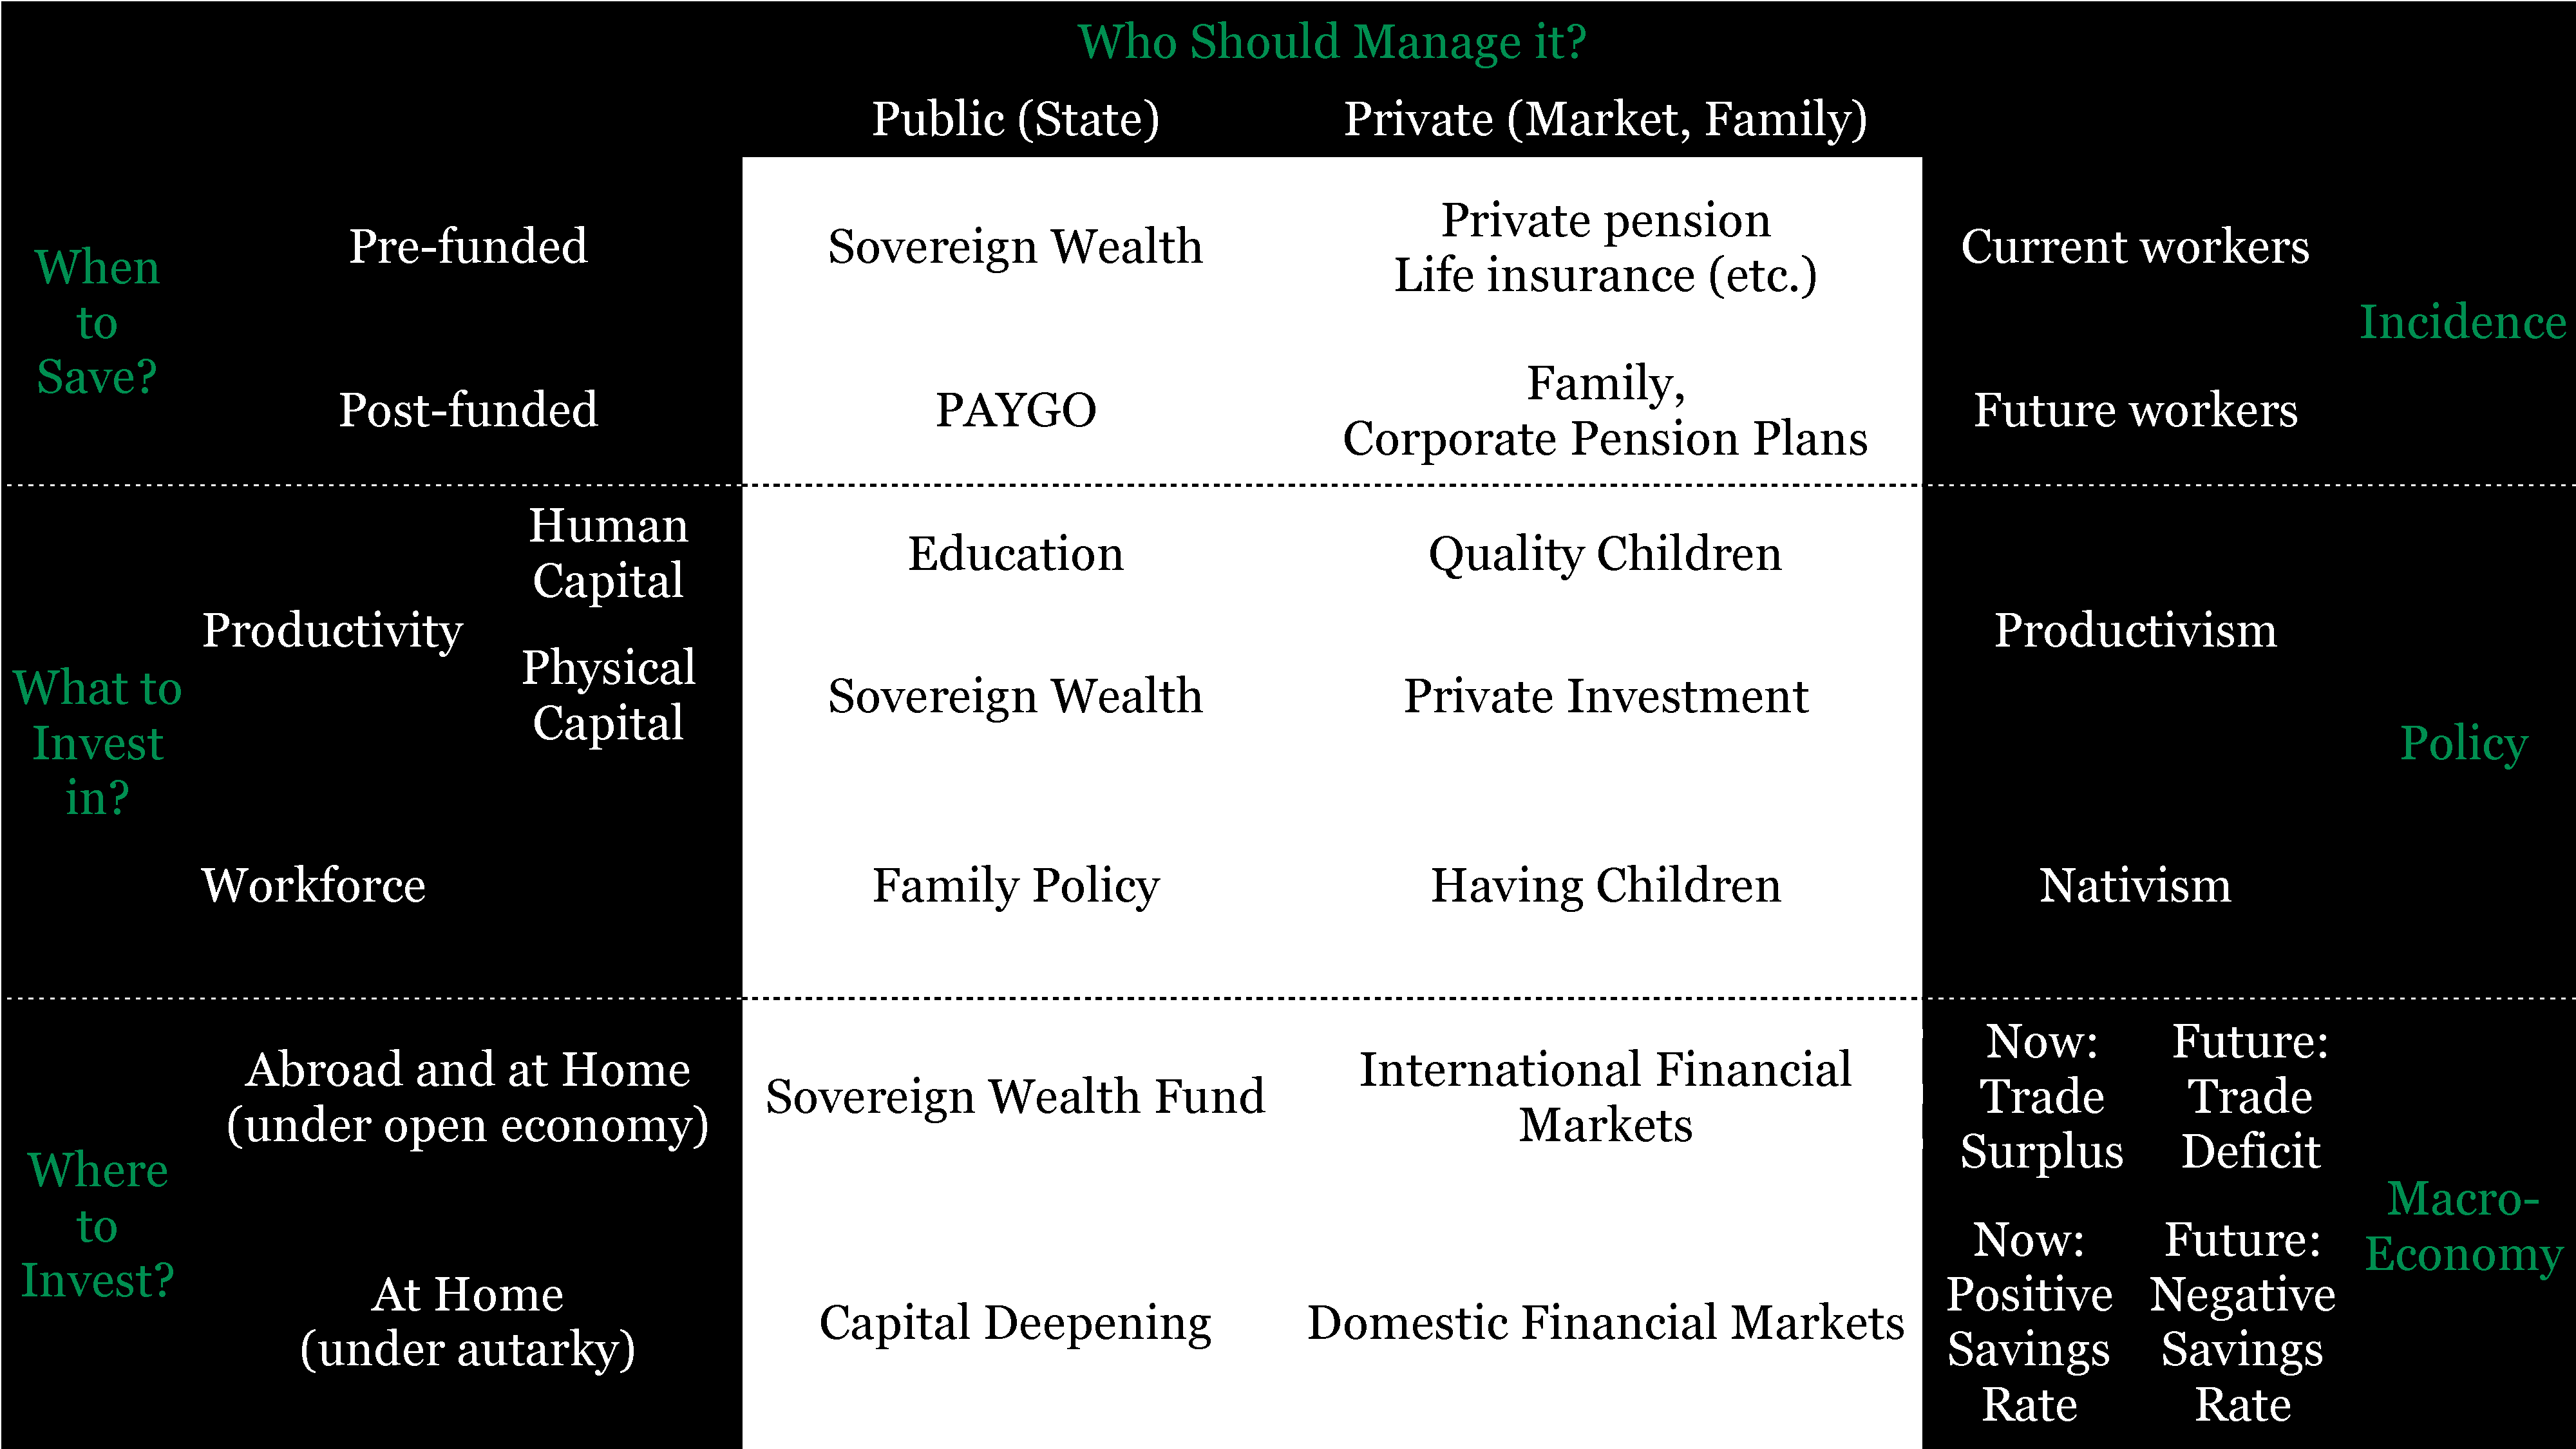
\includegraphics[width=1\linewidth]{pension-design}
	\caption{Pension Design}
	\label{tab:pension-design}
\end{table}%might add family as a third column here.

As summarized in \autoref{tab:pension-design}, all possible pension designs are exhaustively described by tabulating four simple choices:

\begin{description}
	\item[Who Should Manage it?] The surplus production saved for old age can either be managed publicly by the state, including its quasi-fiscal institutions, or it can be managed privately by capital markets (see the the middle two columns in \autoref{tab:pension-design}). In both cases, savers acquire some kind of ownership claim to the accumulated surplus: if under public management, savers own their savings as \emph{entitlements}, governed by public or administrative law, if under private management, savers own their savings as \emph{property}, governed by private law\footnote{
		In \citeauthor{Barr2005a}'s precise formulation, ``PAYGO and funding are both financial mechanisms for organizing claims on that (future) output. (\ldots) Funded schemes are based on accumulations of financial assets, PAYGO schemes on promises'' (\citeyear{Barr2005a}: 157).} \footnote{
		In addition, the right of current savers to future pensions can take the form of \emph{equity} or \emph{debt}. As equity, in either private stock or public economy-wide growth, savers partake fully in both the upside and downside risks: if either the stock, or the economy as a whole grows or falls, so do their pensions. For example, mutual funds share risks under private management and a strict defined-contribution PAYGO-systems share risks under public management. As debt, in either private bond markets or entitlements to future economy-wide incomes, savers are insulated from all but the risk of default. For example, private life insurance includes only a risk of default, and a strict defined-benefit PAYGO-system --- at least nominally --- carries only the risk of sovereign default. \\
		In publicly managed pension schemes, the distinction between the risk profile of equity and debt is often muddled, as future, \emph{nominally} defined-benefit returns are sometimes partly indexed to demographic change, labor incomes, inflation, economic growth or other, risky macroeconomic factors. If and to the extent that such pension schemes turn out to burden future pensioners, instead of future taxpayers or ``social insurants'' with the shortfall, they become de-facto equity investments. \\
		The distinction between equity and debt risk portfolios to publicly managed pension systems carries only so far: in contrast to equity in corporations, equity in sovereigns --- at least ideally --- is always ``non-voting stock''. Conversely, sovereign defaults are different from corporate defaults: in democracies, bondholders \emph{cannot} turn into shareholders and ``take over'' as they would in an insolvent private corporation. The default risk of sovereign bonds is qualitatively different: if a publicly managed pension scheme defaults on its obligations, pensioners can change policy only in their capacity as voters, but, aside from basic rule of law protection, not in any \emph{additional} capacity as bondholders. The bottom line is: if push comes to shove, in publicly managed pension schemes, whether you are a shareholder or a bondholder, your power to change outcomes are mostly those of ordinary voters.}.
	\item[When to Save?] Pension schemes can either be pre- or post-funded. \\
	When they are pre-funded, present surplus production is coagulated into capital \emph{before} future consumption exceeds future incomes in old age. On introduction, current workers bear the initial incidence. Pre-funded pension schemes can be, for example, managed by the state as \glspl{SWF}, or provided by markets as life insurances or other annuities.\\
	When they are post-funded, future income-exceeding consumption in old age is paid out of \emph{future} surplus production of other, younger people. On introduction, future workers bear the initial incidence. Post-funded pension schemes can be, for example, managed by the state as PAYGO, or provided privately in families, or as corporate pension funds\footnote{
		While practically useful, the distinction between pre- and post-funded is mostly nominal, and does not always, in fact, correspond to real savings quotas of an economy. \\
		If pre-funded capital is nominally invested in asset bubbles or other overvalued junk, much of the hard-earned surplus production may actually go to waste and coagulate little in the way form of capital that will actually be valuable, or generate a return in the future. \\
		Conversely, if people are free from such post-funded obligations, but instead use their surplus production to have more children, educate them better, built a home or a company, they \emph{have}, the economy as a whole, does in fact accumulate capital. \\
		In this sense, the current support for pre-funded schemes is based on a false sense of certainty: whether pre-funded pension schemes \emph{actually} stash away enough for old age depends on how good the investments are. The next question, of \emph{How to Grow} is therefore a more meaningful choice than the tiresome pre-funded vs.\ post-funded controversy.}.\\
	\item[How to Grow?] \emph{Any} pension scheme needs to coagulate surplus production somewhere, somehow. Excluding exogenous growth, the long-run output of an economy is determined by the size of its workforce, and the productivity of its workers, which is in turn determined by the different forms of coagulated surplus production they command as human or physical capital, or endogenous technology. Creating both these drivers of output --- people and their productivity --- is costly. The hyper-materialist connotations notwithstanding, creating people or the basis for their productivity are also alternative, competing uses for the surplus of an economy. People and economies can use their surplus production to feed a second baby, or to build a room for the first baby (physical capital), or to better educate the first baby (human capital). \\
	Different pension regimes suggest, and \emph{face} different allocations to generating new workers, and more capital. On the public side, a pension regime may invest surplus production --- pre-funded \emph{or} post-funded --- into better education, or a \gls{SWF}, hoping that either of those will pay off in increased output in the future. Alternatively, a state may try to encourage, and/or individualize the costs and returns of rearing children in its family policy, to increase, or --- better yet --- stabilize future workforces. \\
	On the private side, a private investment may accumulate into physical capital, or family may pour resources into one prodigious child, hoping that both will increase future productivity. Alternatively, a family may decide to have \emph{more} children, hoping that they together, will support the parents in old age.

	\item[Where to Invest?] Lastly, pension schemes can invest their surplus production either abroad and at home under an open economy regime, or, if under autarky, they can invest only at home. Crucially, for private markets, the mix between foreign and domestic investments will be determined by expected returns. Domestic investment can be enforced only if the economy in question foregoes capital mobility and confines itself to --- at least some --- autarky. \\
	These investment choices reflect in macroeconomic movements. A pension scheme investing heavily abroad will first bring a trade surplus, and later, a trade deficit, both set off by respective flows in the capital account. A pension scheme investing only at home will not alter trade balances, but will first build positive savings rates, and later negative savings rates, as the pensions are paid out and consumed away.
\end{description}

%add somewhere a good visualization about pensions, to illustrate the trivial difference between PAYGO and funded. Go back to Barr to figure this out, he's got some good ideas. There's a box in Barr with the economics of pensions that I should look into.

Each of these choices has to be considered very carefully. To name just a few of such vexing considerations, private management might help capital markets mature, and contribute to growth (for example, \citealt{Barr2005a}: 155) --- \emph{or} it might help inflate bubbles, and expose individuals to undue risk. Nativist policy may be considered illiberal, \emph{or} raising children may be considered a positive externality for which parents should be compensated. Investing pensions abroad may be thought to spur growth and convergence, \emph{or} we might find find the colossal --- if ideally only temporary --- trade imbalances unacceptable\footnote{
	Private, pre-funded pension schemes in rich, open economies may cause much capital to flow abroad into emerging economies, where they promise to generate higher marginal returns. In the future, these formerly trade surplus, aging economies such as Germany would then run colossal trade deficits with emerging economies such as Brasil. While many advocate such a scenario (for example, \citealt{Borsch-Supan2003}: 176), I have not read any one remarking on whether such a scenario in which, for example, young Brazilians do much of the producing, and old Germans do much of the consuming would even be conceivable, let alone desirable.}.

The devil, here, as always in policy, dwells in the details, and must be engaged. I allow myself the rather superficial summary in \autoref{tab:pension-design}, because I want to draw attention to the fundamental equivalences of these seemingly dramatic choices: however they answer these questions, pension regimes, as all policy, cannot escape the constraints of Haig-Simons, summarized in \autoref{fig:haig-simons-individual-collective}. If, other things equal, you have fewer children and lower the production of future workers, as Germany presently does, but wish to maintain the standard of living of a future, older Germany and future, older citizens, you \emph{must} invest in either human or physical capital, in some form, by some mean. If,  other things equal, you cut public pension contributions, you have to increase privately managed saving.

The Haig-Simon identity and, as one of its terms, demographic change\footnote{
	The current, second demographic transition (\citealt{Davis1945}, restated by \citealt{Caldwell-1976-aa}) delivered low, often below-replacement level \glspl{TFR} --- the average number of children a woman would have by age 50 based on the current age-specific fertility rates --- and low mortality, concisely measured as life expectancy at birth (after 6 months). \\
	US 2009 estimated TFR: 2.05 \citep{CIA2009}, Germany 2009 estimated TFR: 1.41 \citep{CIA2009}, EU-25 2002 TFR: 1.37 (\citealt{Demeny-2003-aa}: 2). Life expectancy at birth for EU-25 is 69 years for males and 78 years for females (\citealt{Demeny-2003-aa}: 2).},
are unforgiving and inevitable strictures, akin to the law of conservation of matter. Population aging\footnote{
	Falling fertility and falling mortality lead to two interacting effects: the population \emph{shrinks} and \emph{ages}. Pure shrinking alone could ideally be welfare neutral on a per-capita basis. Such pure shrinking with no ageing component would, however, require \emph{rising} mortality as long as TFR is below-replacement level to offset older, larger cohorts.\\
	Ageing, or more specifically, a change in the dependency ratio between very young and very old transfer recipients and everyone else, however, is an unavoidable welfare loss. Fewer people are available to produce for the consumption of more, older people.},
as other real dissavings, harbor unavoidable losses in future welfare (for example, \citealt{Borsch-Supan2003}: 152). They are also both self-reinforcing: dissaved capital not only earns no interest, but also no compound interest, unborn babies not only cannot support their parents, but they also will not have babies, themselves\footnote{
	Demographic shocks echo on for generations and generations, as for example, 1950s baby boomers procreate in the 1970s, and baby-baby boomers procreate in the 1990s, and so on. Population dynamics are so damningly powerful because, as \cite{Malthus1798} knew, it grows geometrically, that is, has an incredibly high ``interest'', and therefore compound interest rate.}.

To these strictures, there really are \emph{no alternatives}, no matter the pension design. There are, however, very real policy choices of whom to burden with the inevitable welfare loss: \begin{inparaenum} \item whether, and to which extent to burden current or future workers, \item whether, and to which extent to individualize the material costs and rewards of rearing children, \item whether and to which extent to tie individual contributions to individual benefits, and, most importantly, \item whether and to which extent to alter the incidence of the pension design through redistributive intervention, that is, taxation. \end{inparaenum}

TINA in the literature on building pension schemes in \gls{CEEC} or reforming them elsewhere, takes a peculiar form. It weighs alternative pension scheme designs, where --- with the exception of devilish details --- there really are no meaningful choices, and neglects those very real choices of burden-sharing that democratic polities have.

\citeauthor{Cerami2009a}, for example, though ever critical of ``neoliberal reforms'', describes extensively the addition of compulsory or voluntary private pensions to \gls{CEEC} regimes and cites demographic change and --- unspecified --- ``economic and financial pressures'' (sic!) as partial reasons (\citeyear{Cerami2009a}: 336).
He seems to forget that the intertemporal Haig-Simons identity of an economy is hardly affected by a privatization of pensions: sure enough, the incidence changes, but no old age crisis can be averted by privatization.
\cite{Barr2005a}, by contrast, are one of the few authors in the field who --- at least implicitly --- endorse Haig-Simons, and exemplarily, reveals the policy options that TINA would have us ignore:
\begin{quote}
	\emph{``An alternative approach [to parametric adjustments] seeks to finance higher future pension spending by reducing other expenditure.
	One way is to reduce public debt now; thus governments in the future would spend less on interest repayments, freeing resources for PAYG[O] pensions''.}
	\\*
	--- \citet[152]{Barr2005a}
\end{quote}

\citeauthor{Cerami2009a} asks for a ``new politics of aging'', involving institutions, ideas and power as a new second-order theory of social change (\citeyear{Cerami2009a}: 338), but, before that, rightly stresses a first-order question: whether, indeed, ``funded'' (by which he means privately managed, pre-funded) pensions really resolve the (unspecified) ``demographic, economic and financial (sic!) pressures'' supposedly arising under ``PAYGO'' (by which he means publicly managed, post-funded) (\emph{ibid.}: 339). There are at least three TINAs that \citeauthor{Cerami2009a}'s account of the first-order social choice falls for:

\begin{enumerate}
	\item \citeauthor{Cerami2009a} (and \citealt{Bastian1998}, too) seemingly accept ``funded'' vs.\ ``PAYGO'' as a demographically meaningful alternatives, even though they are clearly not. Funded, or more precisely, privately managed, pre-funded pensions may change the \emph{incidence} of aging, by burdening current workers, but they not by virtue of being privately managed alter the economy-wide or even individual, intertemporal Haig-Simons identity (for a detailed model see \citealt{Borsch-Supan2003}: 170). Privately managed, pre-funded, just as publicly managed pre- or post-funded regimes may, or may not save enough for the future, and may, or may not invest such surplus production wisely to make up for the dissaving in offspring, and growing life expectancy. ``Pre-funded'' conveys a false sense of austere security that social scientists should not buy into.

	\item Likewise, \citeauthor{Cerami2009a} cites, without reproach, the arguments for ``pre-funded'' schemes, including supposed higher returns of private investments and breaking of the ``vicious cycle'' of PAYGO. Both, again, assume alternatives where there truly are none.

	Privately managed funds may, or may not generate higher returns than equivalent \glspl{SWF}. Any supposed superior performance of one or the other management requires a specific economic theory to explain it, and empirical evidence to support it, non of which are mentioned here\footnote{
		There may be good, theory-driven, empirically supported reasons for favoring private or public management of pre-funded schemes, but that is part of the messy detail that neither \citeauthor{Cerami2009a} nor I can, or need to discuss here.}.
	To just mention such supposed superiority of privately-managed funds without explaining why that would be so, is to buy into the unquestioned promises of neoliberal ideology.

	There is also no such thing as a ``vicious cycle'' of PAYGO, where, in \citeauthor{Cerami2009a}'s reading of its opponents, ``current workers are forced to pay for current pensioners'' (339). True enough, a move from nominally post-funded to nominally pre-funded regimes alters the nominal incidence of demographic change, but that is simply a zero-sum redistribution of the hardship that some group, at some point, has to endure. There is nothing particularly self-reinforcing about (nominally post-funded) PAYGO, that would make it ``vicious''.

	A similar notion comes from \cite{Bastian1998}, who, with alarm, reports the rising share of public pension outlays in \gls{CEEC} GDP (\citeyear{Bastian1998}: 69), and cites PAYGO as the ``main reason'' of the fiscal malaise (\emph{ibid.}: 71). That is of course, rather tautologically, true: in a PAYGO system, all other things equal, the public purse absorbs demographic change. However, he seems to be unaware that the percentage of pensions, or, equivalently, consumption of elderly people, is entirely \emph{invariant} to the pension design. If PAYGO is transformed into a ``funded'' scheme, the same number of old people will, all other things equal, still consume the same percentage of economic output.

	\item Conversely, \citeauthor{Cerami2009a} also glosses over the arguments presented against pre-funded reform.

	He reports caution about the supposed demographic cure-all of pre-funded pensions (339), but again, fails to explain why --- as is in fact correct --- the public or private management, or even nominal pre- or post-funding do not alter the Haig-Simons dissaving at all.

	\citeauthor{Cerami2009a} also cites risks associated with unstable markets (339) as evidence for the prosecution of pre-funded schemes, but apparently relying more on leftist gut-feeling than critical reasoning, fails to explain what the theory and evidence of theses risks would be. To be sure, pension schemes should probably spread and thereby minimize risk, but as these messy details go, they are no matter to be mentioned in passing. \citeauthor{Cerami2009a} here assumes a possibly non-existing alternative by suggesting that \emph{only} privately managed, pre-funded pension schemes are risky. Clearly, publicly-managed, even post-funded pensions also include --- albeit probably smaller\footnote{
		\ldots or not, according to \citealt{Borsch-Supan2003}: 178.}
	--- risks: an \gls{SWF} can make poor investments, and even a social-security PAYGO system by only betting on one class of investment (labor productivity) in one market (the domestic economy) takes on risks\footnote{
		For example, \citeauthor{Cerami2009a} presents  2009 \gls{OECD} reports of 20\% losses in private pension funds as evidence against private management. That need not be so: \begin{inparaenum}
			\item The losses may so far be evident only in balance sheets, and need not ever --- but well may --- materialize in diminished cash flows. The depreciated assets may bounce back. Well-managed funds will insulate individual pensioners from such short- and medium-term fluctuations. \item These same losses, might, absent a private pension scheme, have materialized elsewhere in the economy. For example, workers might have invested the windfall in other risky assets. Bubbles and crashes are inter temporal bumps in the Haig-Simons identity, and they will always hurt the economy --- as \citeauthor{Cerami2009a} (340) concedes ---, no matter their nominal incidence.\end{inparaenum}}.
	Pensions --- as all savings --- always entail some risk: whoever manages this pre- or even nominally post-funded surplus production has to decide where it will generate the highest return at an essentially uncertain future point in time. As \citeauthor{Barr2005a}, again lucidly, point out: ``PAYG[O] and funding are both financial mechanisms for organizing claims on that [future] output [\ldots] [and] fare similarly in the face of output shocks.'' (\citeyear{Barr2005a}: 156).

	But \citeauthor{Cerami2009a} here also ignores an alternative, that in fact may exist: well- (or better-)regulated markets that efficiently spread, and thereby minimize risks. Especially to a critical social scientists there must be a very good reason to assume that financial markets are \emph{always} unable to spread risk, or, absent such compelling (economic, first-order) reason, the social scientist must suggest (sociological, second-order) reasons why the institutions of financial capitalism underperform in this specific way. By not even alerting us to this issue, but by dogmatically assuming financial market failure, \citeauthor{Cerami2009a} --- surely unintentionally --- feeds a particularly backhanded TINA of truly neoliberal hegemony: that financial markets --- be they good or bad --- cannot be altered, or, that their failure or success is inevitable, and needs no social scientific explanation\footnote{
		For a fully-fledged Gramscian account of european integration, see \cite{Bieler2002,Bieler2003,Bieler2005}.}
	%make sure to mention risk in the above.

	Lastly, as an inverse argument to the ``vicious cycle''-critique of PAYGO, \citeauthor{Cerami2009a} cites the ``double payment'' of current workers as they are transitioned to a pre-funded regime\footnote{
		As a pre-funded, privately managed component replaces, or is added to a nominally post-funded, public managed pension, current workers have to pay twice: once into a private account for their old age, and once into a public account fur currently old, PAYGO recipients.}.
	As the ``vicious cycle'', the ``double payment'' argument is mis-construed: there is \emph{nothing} particularly bad, or ``double'' about pre-funded regimes, just as there is nothing ``vicious'' about post-funded regimes. The difference between the two is a trivial, zero-sum redistribution of the incidence of demographic change. Under PAYGO, depending on parametric configurations, the young and/or the old pay for the dissaved future workforce. When pre-funded regimes are added to the mix, but all other things remain equal, only the young pay for demographic change. The sum paid, in any event, does not change. By framing pension reform as a struggle between the currently young and the currently old, \citeauthor{Cerami2009a} falls for an old ruse: \emph{divide et impera}, divide and conquer. If we obsess about the mystically ``vicious'' or ``double'', but truly trivial incidence of pre-funded vs.\ nominally post-funded pensions, we loose sight of the bigger redistributive choices of aging societies: whether to burden the rich, or the poor, to burden current, or future generations.
\end{enumerate}

It may, again, seem nitpicky, to relentlessly criticize authors as critical as \cite{Cerami2009a} himself, who, after all, only reports arguments frequently presented. Still, I (nit-)pick on \citeauthor{Cerami2009a}, precisely because he is so far left of neoliberalism, but, I would maintain, not persuasively so. He rightfully alerts us to the ideological import in pension reform debates (\emph{ibid.}: 340), but penetrates not nearly deep enough into the economic abstractions of pension-design to fully expose the hegemony he correctly suspects. Whatever the merits of his second-order \emph{explanans} of a new politics of pension reform, he has the first-order \emph{explanandum} wrong: he assumes economic alternatives where there are none (pre-funded vs.\ post-funded), and neglects other, more relevant choices (financial market reform).

TINA plagues not only the right, but, more deviously, the left, too. When critical social scientists, as \cite{Cerami2009a}, present only the dogmatic, but shorthanded arguments against neoliberalism (``private pensions are too risky''), their important dissent remains superficial, and will easily brushed aside by more assiduous, if duplicitous, neoliberals.

TINA operates not by straightforwardly denying leftists ``possible, better worlds''. Rather, TINA is neoliberal and conservative in a roundabout way: it obfuscates the abstractions through which any such hypothetical, preferable worlds may be glimpsed.
And so, even critics as \citeauthor{Cerami2009a}, inadvertently serve TINA, when they neglect the deep economic abstractions, maybe confusing their neoclassical language and hard choices for the neoliberal doctrine that has so successfully appropriated them. In pension design, as elsewhere in public policy, a Haig-Simons understanding of the economy helps us to sift through the epiphenomenal debates (``funded'' vs.\ PAYGO), to relegate the complex details (financial markets) to appropriate theory and data, and advance to those choices that our scarce, constrained and material world leaves us to take: how much we should save for future generations and in which form, and who of us, rich or poor, should contribute how much. \emph{These} are the real first-order alternatives that a second-order theory as \citeauthor{Cerami2009a}'s must take as a starting point. All policy and all pension designs, underneath the complex detail and nominal casuistry, make these choices. My hunch is: many  current designs and their marginal reforms greatly burden future generations, and present non-rich people, a peculiar choice, that may not even enjoy popular support.

\citeauthor{Schui2009} is right to point out that minimizing the problems of old age insurance to demographic change is latently affirmative: it distracts us from the possibility to redistribute the fruits of growth and the pains of decline (\citeyear{Schui2009}: 147)\footnote{
	\citeauthor{Schui2009}, the orthodox leftist, is of course otherwise hardly moved by the strictures of Haig-Simons. Ever the die-hard Keynesian --- or Marxist? ---, he always and everywhere assumes a crisis of underconsumption, or, equivalently, excessive overall profits, and seems not to allow even the possibility of material constraints at some exogenously given, only slowly expanding steady state.}.

The enormity of these alternatives can hardly be overstated, especially for \gls{CEEC}, where hard-working people often spent old age in abject poverty. As even the aging economies of Europe \emph{are still growing} over the medium- and long-term on a per-capita basis, we should be able to build a pension regime that, somehow\footnote{
	Progressive taxation comes to mind.} \footnote{
	A pension scheme including, or supplemented by progressive taxation, does not preclude actuarial components in a pension formula. As \cite{Barr2005a} helpfully reminds us, working longer may not be such an undue thing to ask, if people live longer, too. If people some people like to retire earlier, and others are willing to work longer, we might want to punish and reward them accordingly, while still asking the rich to chip in more for any actuarial increment earned. Alternatively, and probably more transparently, the redistributive component can also be organized exclusively through the tax code, with pensions remaining cleanly actuarial.\\
	Evidently from the summary of the mixed economy in \autoref{tab:ends-mixed-economy} (p.~\pageref{tab:ends-mixed-economy}), if, regrettably, not from all real existing self-ascribed social market economies, asymmetrically known \hyperref{sec:risk}[risk] should be covered by compulsory or state insurance. This also includes disabilities that may occur more often in old age, or in some occupations. Presently, some pension regimes --- clumsily --- include some form of old-age disability insurance, and debates on extending the age of retirement inevitably bring up the plight of the old construction worker. In all of this, I assume that there is extensive, compulsory or state-covered disability insurance. When I argue for actuarial pensions, and/or later retirement, I assume that whoever cannot, because of occupational or other disability, work into her older age, should receive benefits out of the disability insurance until she reaches the statutory retirement age. If, as seems likely, disability clusters in risky or hard jobs --- such as teaching or construction --- it may even make sense to charge a premium for insuring these jobs, so as to raise the costs of such hazardous labor, and to make it safer or rarer.}
collects this still increasing economic output, saves enough for our children and disburses enough to our seniors.

If we do not, such criminal neglect of the mixed economy certainly deserves a fair trial, and begs a social scientific explanation.

%barr, for pensions is the benchmark \cite{Barr2005a}

\subsubsection{Pangloss} \label{sec:Pangloss}

\begin{quotation}
	\emph{``It is demonstrable'' said he, ``that things cannot be otherwise than they are; for as all things have been created for some end, they must necessarily be created for the best end.
	Observe, for instance, the nose is formed for spectacles; therefore we wear spectacles.
	The legs are visibly designed for stockings; accordingly we wear stockings.
	Stones were made to be hewn and to construct castles; therefore my lord has a magnificent castle; for the greatest baron in the province ought to be the best lodged.
	Swine were intended to be eaten; therefore we eat pork all year round. And they who assert that everything is right, do not express themselves correctly; they should say that everything is best.''}
	\\*
	--- Fictional Dr.\ Pangloss in Voltaire's novella \emph{Candide} (\citeyearpar[loc.~125]{Voltaire1759}
\end{quotation}

\paragraph{Second Best.} Today, maybe one of the clearest Panglossian pronouncements comes under the imposing heading of a \emph{Theory of Second Best}, originally formulated by \cite{Lancaster1956}. As so many great economic ideas, this one has strayed far from its original form, and interbred with ideology to father many illegitimate --- and sometimes  deformed --- offspring.

In its initial, rigorous formulation, the Theory of Second Best showed formally that if --- as seems likely --- some conditions for the pareto optimality of markets cannot be meet, it might enhance efficiency to allow additional, possibly offsetting deviations from perfect competition elsewhere in the economy. Rather than to fight all market failures everywhere in isolation (``piecemeal welfare economics'', \emph{ibid.}: 11), \citeauthor{Lancaster1956} suggested that from a general equilibrium view, there may be less demanding \emph{necessary} conditions that could pareto improve the economy, in addition to the often implausible, \emph{sufficient} conditions of perfect competition (\emph{ibid.}: 17).  \cite{TheEconomist2007} explains it beautifully thus: if your optimal cookie recipe requires chocolate chips and coconut flakes, but you cannot find the chocolate chips, your (second) best bet may be to bake gingersnap, rather than chocolate chip cookies without chocolate chips. This is the kind of devilish complexity that I allow myself to ignore here, but that policy makers have to consider: if, for example, research and development are so prohibitively expensive that we absolutely cannot profitably have more than one manufacturer of wide-body aircraft, our (second) best policy may indeed be to stray further from neoclassical doctrine, and to keep subsidizing \emph{The Boeing Company} and \emph{Airbus SES}, so that we can have at least have ourselves a decent, somewhat competitive, duopoly. There is nothing Panglossian about such hard choices because, it is, in fact, \emph{materially} impossible to develop dozens of competing wide-body designs. Because for the social sciences --- as for moral philosophy --- \emph{ought implies can}, the second-best of the subsidized Boeing/Airbus duopoly also needs no social scientific explanation. This \emph{really} is collateral damage to a worthy cause.

After \citeyear{Lancaster1956}, however, the Theory of Second Best as slowly morphed into a general skepticism of state intervention, it is now name-dropping ``proof'' of its \emph{ipso-facto} futility and serves as welcome absolution for the demise of the mixed economy. \citeauthor{Wolf1987}(\citeyear{Wolf1987,} \citeyear{Wolf1979}), for example, argued that because governments fail, just as markets do, the second-best response to such market failures may be to just let them be. You can take this argument to merely logical extremes, and throw out government and democracy altogether. \cite{Leeson2009}, for instance, wonders whether in some (developing economies) settings, anarchy may not be preferably to predatory statehood, whether, in other words, no state would not be second-better than an inevitably failing government. \cite{Caplan2007}, in an otherwise thoughtful book, seems to suggest that because voters are so invariably rationally irrational, markets may be second-better than democracy altogether.

This has very little to do with the rigorous argument presented by \citeauthor{Lancaster1956}: he did, at least in \citeyear{Lancaster1956}, never consider a constrained government, let alone an incapacitated democracy to be grounds for ``second-besting'', but, instead even seemed to hope for a government and people powerful and wise enough to heed his call.

This is Pangloss at his finest: if you assume, as modern-day second-besters do, that the very \emph{means} to deliberately get to a better world --- government and democracy --- are inevitably flawed, you can show, with almost hermetic logic, that whatever world we find ourselves in, must be the best of all \emph{possible} worlds.

In that word --- possible --- lies the catch. Modern-day second-besters assume that, akin to markets and evolution, government and democracy are \emph{aimless} processes that merely aggregate pre-social, more- or less rational self-interest. If government and democracy are aimless, it follows --- as it does, in fact, follow for markets and evolution --- that any positive results of government and democracy are beyond reproach, and beyond improvement. Government failures, as monopoly pricing or an appendicitis, are just \emph{facts}.

%Interesting criticism of "more market". Do they really create "stronger incentives to both acquire information and 	evluate it rationally" (272)? See: financial crisis! (Ok, will need to argue this in great care, talk about Keyne's beuaty context. There was some state in causing the financial crisis. Ok, Somin points out that whatever the flaws of markets, market actors may have MORE of an incentive to inform themselves than voters. This may be correct.
	%Somin is a naysayer of deliberative democracy. A pessimist. She doesn't look into the essential innovation of DD!
	%However, this is a deeply broken argument. We should decide on first-best, welfare economic grounds which decisions are a subject to democractic rule, and which are not. We shouldn't have to factor in the inability of democratic systems in this logic.

Enlightenment, the mother of modern science, did not consider democracy, a merely \emph{positive} affair, but a normative prescription. \cite{Kant1785} asked us not to ``follow your incentives'', but to ``act only on that maxim through which you can at the same time will that it should become a universal law'' (\emph{ibid.}: Chapter 11). The US Constitutional Convention in 1787, did not just decide to try out this new \gls{FPTP} way to aggregate preferences, but ``We the People'' were to do so ``in Order to form a more perfect Union''.
In a free society, social scientists need not believe in these, or any other ideas, but if they reject them all, they deserve not the air of scientific sophistication in which they cloak their utter cynicism. As mere accountants of the status quo, their work is anathema to Enlightenment, and they ought to be disowned of the emancipatory heritage that the social sciences were endowed with.

But ignoring, for now, the enlightened humanism that comes part and parcel with the social sciences, the logic of modern-day second-besters is also simply fallacious. Even if government and democracy turn out to inevitably disappoint, such flaws are \emph{not}, to the social scientist, quasi-material constraints. Because government and democracy \emph{are} the subject matter for the social scientist, she must not presume, but has to \emph{explain} them. If we do, as the second-besters, exclude from the first-order alternatives to be explained by second-order theory, those alternatives that the political process \emph{may} corrupt, we have thereby conflated first and second-order theory. Whatever second-order theory might have to tell us about a corrupted political process, we would never learn, if we did not test for the absence of first-best solutions. This Frankenstein variant of the Theory of Second Best confuses, as \cite{Brubaker-2002-aa} succinctly criticized the literature about ethnic conflict, the ``empirical data'' with our ``analytical toolkit'': government failure is ``what we want to explain, not what we want to explain things \emph{with}'' (\emph{ibid.}: 165, emphasis in original).
%add caveat to this, excusing the guy on development second best that indeed, government failure may be endemic under some constellations.

Panglossian bastards of the Theory of Second Best also roam the literature on European and \gls{CEEC} welfare states. I will here only cite one model student of Pangloss', and eminent social scientist, \citeauthor{Moravcsik-2002-aa}, who refutes a supposed neoliberal bias of european integration thus:
\begin{quote}
	\emph{``No responsible analyst believes that current individual social welfare entitlements can be maintained in the face of these [postindustrial, demographic, etc.] shifts.
	In this context, the neo-liberal bias of the \gls{EU}, if it exists, is justified by the social welfarist bias of current national policies [\ldots].''}
	\\*
	--- \citet[618]{Moravcsik-2002-aa}
\end{quote}
%add here
In other words, even if European integration constrained national, democratically governed mixed economies, that would be for the better because these welfare states are too spendthrift to begin with. Also, according to \citeauthor{Moravcsik-2002-aa}, to suggest that mixed economies might --- using efficient fiscal, regulatory and monetary tools --- alter market allocations any which way they want, is \emph{irresponsible}. Pangloss would probably applaud how elegantly \citeauthor{Moravcsik-2002-aa} defines away all redistributive considerations, and, for good measure, adds an ad hominem.

\paragraph{En- or Retrenchment.} Todays Pangloss has grown more sophisticated since the times of Enlightened Absolutism, when he was easy game for satirist Voltaire. As any influential teacher, he has learned to lead on his students by making them ask the questions that suit his lesson plan. The lesson relevant here is that on European and \gls{CEEC} welfare states. It is remarkable just what kind of feeble questions our ever-affirmative teacher Pangloss has gotten us to ask.

\cite{Beckfield2006}, for instance, contents himself to ask how much of \gls{EU}-15 income inequality can be explained by regional political integration as opposed to (economic) globalization, and, alarmed, finds that nearly half of it can be explained thus. He lists the ways in which  regional political integration constrains the welfare state: through \begin{inparaenum}
	\item policy feedback such as austerity-enforcing nominal convergence criteria,
	\item diffused classical-liberal policy scripts
	\item possible blame avoidance and
	\item by tying \gls{MS} economic fortunes to one another.
\end{inparaenum} This is rigorous empirical work, albeit, lacking a natural experiment, and plagued by questionable external validity and --- one fears --- intricate multicollinearity, it will always remain vulnerable to methodological critique. More important, though, is what \citeauthor{Beckfield2006}, in his quest to tell apart the inequality of globalization and political integration, \emph{does not ask}: how much of the rising income equality could an intact, european mixed economy have enforced, and why did it not do so? The bigger question, I would maintain, is what \emph{kind} of political integration could have curbed inequality. \citeauthor{Beckfield2006}, again, surely is one of the authors rightfully critical of globalization and the current mode of \gls{EU} integration. Still, Pangloss, one imagines, sympathetically smiles at this diligent student, hardly moved in his affirmation of the status quo by such timid and naive questions. Pangloss can rest assured, as long as \citeauthor{Beckfield2006} and others busy themselves with the nitty-gritty of welfare state retrenchment, nicely playing globalization off against regional integration, which are really two sides of the same coin. Ever affirmative, if pressed for an explanation, Pangloss can still wring his hands at the inequality, shrug his shoulders and point to the gains from trade. He has already won this game, as \citeauthor{Galbraith2002a} wryly observes: ``So what are the facts [of inequality]? Has globalization hurt or helped? Oddly, researchers do not know; mostly they do not ask.'' (\citeyear{Galbraith2002a}: 11, also \citealt{Crouch2004}: 158).

If sceptics as \citeauthor{Beckfield2006} are the slightly recalcitrant, but still manageable students in Pangloss' classroom, the naysayers of retrenchment as \cite{Swank-2005-aa} are his overzealous disciples. \citeauthor{Swank-2005-aa} argues that globalization did not force welfare states to retrench, because, evidently, income replacement rates in unemployment, health and pension insurance remain high. Pangloss would surely applaud in delight: ``excellent work, all is well!''. What did \citeauthor{Swank-2005-aa} \emph{not} ask, that would so endear himself to Pangloss? Plenty.
\begin{enumerate}
	\item Obviously, and at minimum, \citeauthor{Swank-2005-aa} should look at public debt and other \hyperref[sec:smoke-n-mirrors]{smokes and mirrors} of the mixed economy to make sure that these sustained income replacement rates are not built on a base of sand, long washed out by tax competition (p.~\pageref{sec:smoke-n-mirrors}). He is certainly right that there will be substantial political pressure to maintain welfare states, but their victories may be pyrrhic if bought at the price of sovereign default, or heightened \glspl{DWL}.
	\item More fundamentally, the causal rejection (!) of welfare entrenchment through globalization as put forward by the optimists needs careful positivist research design.  This would require a hypothetical, namely a sufficiently large, prosperous and closed economy. This does not exist in the OECD world, and may not exist at all in reality, as there is a well acknowledged trade-off between liberalization and prosperity. This real world constraint notwithstanding, empirical arguments have to take this methodological problem into account to answer the question whether welfare states can \emph{sustainably} continue to operate under international economic liberalization.
	\item Thirdly, lastly, and most fundamentally, the optimists seem to be not so much optimistic about what a welfare state can do, as they seem to be minimal about what it should do. In part, this neoliberal bias follows from an epistemological concentration on the status quo. The research question that \citeauthor{Swank-2005-aa}, for example answers, is not whether globalization challenges the welfare state. Instead, he argues that it may not affect the status quo of \emph{income replacement}. This is an unexplicated, negative and minimal definition of the welfare. It assumes that the legislator’s social agenda is limited to income replacement, without regard to broader redistributive issues, particularly the question of who should bear the costs of income replacement. More generally put, this amounts to what the public management literature calls an output perspective on how much money is spend on welfare, in this case.
\end{enumerate}

% More generally put, this amounts to what the public management literature calls an output perspective on how much money is spend on welfare, in this case \marginpar{\textsf{(reference)}}. Much akin to (absurdly) treating anti-discrimination policy, however extensively defined, as an instance of social policy
%proper \citep{Leibfried-2005-aa}, accepting income replacement as a meaningful dependent variable of welfare retrenchment, reveals the neoliberal bias of this strand of optimistic arguments. Income \emph{replacement} already by name, is negatively defined, and diminishes social policy to be concerned with the abolition of negative constraints (hardship from unemployment), of things we cannot do and, at the same time clouds a positive definition of social policy as furthering our freedom \emph{to} do something, not freedom \emph{from} something.

%Welfare regimes are, as \cite{Esping-Andersen-1990-aa} has said, systems of stratification in itself \marginpar{\textsf{(page)}}, and they have been, from the very beginning socialist demands in the 19th century more than epiphenomenal income replacement. They are tools to socialize the costs of painful, but welfare-enhancing Schumpeterian \marginpar{\textsf{(reference)}} economic transformations as well as individual hardship and serve as engines to redistribute this very welfare as the legislator wishes.

%\subsection{The Right Hypothetical}

%The indeed quintessential and highly political question for globalization and welfare entrenchment is then, whether the state can still socialize and redistribute as it wants, with no limitations resulting from the behavior of other states. Welfare state sustainability then has to be pitted not against past or current performance, but against a hypothetically desired welfare regime under global trade with global redistribution, both within and between countries.

%\subsubsection{The Missing Cell in the Payoff Matrix} In game theoretic terms, to gauge how badly welfare-depressing defection might be, you first have to calculate the payoff of a hypothetical mutual cooperation.

%\begin{table}[htbp]
%  \small
%   \begin{center}
%\begin{tabular}{m{1cm}m{2,3cm}m{2,3cm}m{2,3cm}m{2,3cm}}
%& & \multicolumn{3}{c}{\emph{Rest of World}} \\
%& &Open Markets $\wedge$ High Taxes & Open Markets $\wedge$ Low Taxes & Autarky  $\wedge$ Any Tax \\
%\cline{3-5}
%\multicolumn{1}{c}{\multirow{6}{*}{\emph{Home}}} & \multirow{2}{2,3cm}{Open Markets $\wedge$ High Taxes} & \multicolumn{1}{|r|}{?} & \multicolumn{1}{r|}{$x\geq2$} & \multicolumn{1}{r|}{0}\\
%\multicolumn{1}{c}{} & \multicolumn{1}{c}{}& \multicolumn{1}{|l|}{?} & \multicolumn{1}{l|}{$x\leq2$} & \multicolumn{1}{l|}{0}\\
%\cline{3-5}
%
%\multicolumn{1}{c}{} & \multirow{2}{2,3cm}{Open Markets $\wedge$ Low Taxes} & \multicolumn{1}{|r|}{$x\leq2$} & \multicolumn{1}{r|}{2} & \multicolumn{1}{r|}{0}\\
%\multicolumn{1}{c}{} & \multicolumn{1}{c}{}& \multicolumn{1}{|l|}{$x\geq2$} & \multicolumn{1}{l|}{2} & \multicolumn{1}{l|}{0}\\
%\cline{3-5}
%
%\multicolumn{1}{c}{} & \multirow{2}{2,3cm}{Autarky $\wedge$ Any Tax} & \multicolumn{1}{|r|}{$0< x\geq$ ?} & \multicolumn{1}{r|}{$0< x\geq2$} & \multicolumn{1}{r|}{0}\\
%\multicolumn{1}{c}{} & \multicolumn{1}{c}{}& \multicolumn{1}{|l|}{0} & \multicolumn{1}{l|}{0} & \multicolumn{1}{l|}{0}\\
%\cline{3-5}
%
%\end{tabular}
%\end{center}
%   \scriptsize{The above payoff matrix is not a well-defined, sufficiently formalized game. To adequately model the international political economy, \emph{Rest of World}, ROW, would have to be disaggregated into at least two more players, making a two-dimensional representation of the game impossible. Liberalization and taxation are impossible to  be adequately modeled with only two players, for then, autarky of one player would by definition imply autarky of the other player. In real life, at least theoretically, countries could exit from international trade and finance with other countries still continuing on the road to liberalization.}
%   \caption{A Schematic Payoff Matrix for the International Political Economy of Taxation and Liberalization.}
%   \label{tab:SchematicPayoff}
%\end{table}
%
%\marginpar{\textsf{Quite a bit of thinking, reading is still required for the below.}}
%
%\autoref{tab:SchematicPayoff} shows a schematized payoff matrix of the international political economy of taxation and liberalization\footnote{A number of other qualifications and complications do not feature in this schematic overview. The high-vs.-low-tax dichotomy does not take into account the above-mentioned shifts in tax bases and progression, namely to more indirect, regressive taxation which may more closely approximate the actual dynamics of tax competition. Likewise, the game between \emph{Home} and \emph{ROW} assumes equal sizes of the two economies and cannot account for differential payoffs depending on country size, that \cite{Dehejia1999} have recently pointed to.}.
%
%\paragraph{You Gain from Trade} Firstly, it assumed here that autarky is always the worst outcome\footnote{The effects of autarky of \emph{Home} on \emph{ROW} crucially depend on the respective sizes of the two economies. If \emph{Home} is sufficiently large, it may cause \emph{ROW's} payoff to approximate zero. Alternatively, if \emph{Home} is small, its influence on \emph{ROW} will be negligible, and \emph{ROW's} payoff will approximate what it would have been otherwise. This result is equivalent to disaggregating the unrealistically uniform actor \emph{ROW} into an n-player game, where the choice for autarky of every single player has a negligible impact on others.}. Dynamic effects of protectionism, including infant industry development, are not considered here.
%
%\paragraph{You Lose from Taxation --- Or Not} Secondly, it is assumed, that if one player has relatively lower taxes on open markets, that player will attract same or more factors of production and therefore receive a same or higher payoff. The counterparty will receive same or a lower payoff, respectively. The empirical picture regarding this payoff is mixed; the above-mentioned optimists seem to suggest that costs of higher taxation --- if they are considered at all --- do not cause significant capital flight \marginpar{\textsf{(references)}}. More pessimist analysts suggest, that in fact, relatively higher or more progressive taxation, for example of corporate incomes causes factors of production to move, and thereby payoffs to diminish \cite{Genschel2009} \marginpar{\textsf{(and more references)}}. I have therefore assumed that payoffs under higher taxation will diminish or stay same.
%
%\paragraph{Rational Actors Will Play It Safe} Assuming that nothing, not even a probability distribution is known about the outcomes of mutual high taxation, mutual low taxation emerges as a dominant strategy for both players. From every other course of action, independent of the behavior of the counterparty, players stand to loose, stay same or receive an unknown payoff. Risk-averse actors will converge on mutual low taxation as the Nash Equilibrium.
%
%\paragraph{Empirical Investigation of the Status Quo is Futile} From this analysis emerges a fundamental limitation to empirical investigations of the status quo. If we accept that unilateral high taxation will create same or lower payoffs, further assume that that this fact is widely known by rationally acting states, it is logically impossible to gauge whether \emph{in fact}, higher taxation is costly, and if so, by how much. For no matter how high these costs are, or whether they in fact would be incurred, we cannot know about them.
%
%The nature of the game is then indeterminate. We cannot ascertain from what we observe whether there are gains from cooperation to be harvested. We cannot know how much we loose from tax competition, for we cannot see how deep down that putative vicious cycle we already are.
%
%To solve this game, we have to compute a hypothetical payoff for uniform high taxation. If that payoff is higher than the currently achieved one --- as is hypothesized here --- and if states behave rationally (!), we then have a strong reason to assume that payoffs for unilateral high taxation are smaller.
%
%Without that hypothetical hypothetical of uniformly high taxation, any attempts to solve the game are marred with a fundamental endogeneity problem.
%
%\subsubsection{Dream \emph{On}, Policy Analyst!}
%
%Even leaving normative considerations aside, as I have tried to demonstrate in the above, just academic rigor alone requires us to hypothesize a hypothetical of a globalized, uniformly taxed world economy.
%
%This certainly requires quite a bit of political imagination, something that political scientists, it appears, like to shy away from. The question that economists, political scientists and law students in this field have to answer really is a very basic one that has fallen into disrepute under a misunderstood fetishizing of ``disinterested science''.
%
%Put emphatically, to know whether this world is \emph{the best of all worlds} --- or just why it would not --- a certain amount of dreaming how it \emph{could} be better is not only allowed, but analytically require. It is hard to learn just \emph{how much} present conditions constrain us, without assuming them away.
%
%To sum up: explaining why the world is not different (in this, case better), ought to serve the classic Popperian business of disconfirming just as well as showing why it is the way it is, or why it is not worse.

%check this again! Not sure about Leibfried!
%!marginpar!
\marginpar{The remainder of this section is still quite confused. It needs a better structure and I need to double-check the references. Read with care.}

But Pangloss is pleased with other students, too, including such eminent voices as \cite{Leibfried-2005-aa} who seems to consider anti-discrimination policy as an instance of social policy proper. Pangloss might silently rejoicing at the neoliberal bias he has so successfully instilled in his student. Anti-discrimination --- however extensive --- already by name, is negatively defined, and diminishes social policy to be concerned with the abolition of negative constraints, of things we cannot do, of market distortions and at the same time clouds a positive definition of social policy as furthering our freedom \emph{to} do something, not freedom \emph{from} something.

Welfare regimes are, as \cite{Esping-Andersen-1990-aa} has said, systems of stratification in themselves, and they have been, from the very beginning socialist demands in the 19th century more than epiphenomenal income replacement. They are tools to socialize the costs of painful, but welfare-enhancing \citeauthor{SchumpeterSwedberg-1942-aa}ian economic transformations as well as individual hardship and serve as engines to redistribute this very welfare as the legislator wishes. The indeed quintessential and highly political question for globalization and welfare entrenchment is then, whether the state can \emph{still} (or ever could) socialize and redistribute as it wants, with no limitations resulting from the behavior of other states. Welfare state sustainability then has to be pitted not against past or current performance, but against a hypothetically desired welfare regime under global trade with global redistribution, both within and between countries. In game theoretic terms, to gauge how badly welfare-depressing defection is, you first have to calculate the payoff for mutual cooperation.
In the global context, this certainly requires quite a bit of political imagination, something that political scientists, it appears, like to shy away from. Even leaving normative considerations aside, in this case, academic rigor alone requires such exercise.

If welfare states can be well or poorly designed mixed economies, achieving different outcomes, we should also judge its prospects by comparing actual or evolving regimes to such hypothetical, but possible and desirable configurations. That is a very different question than testing whether welfare states en- or retrench, let alone its spurious correlates of income replacement \citep{Swank-2005-aa} or even spending (\citealt{Kleinman2002}: 24), and a question that would deeply unsettle Pangloss. As \citeauthor{Offe2003} reminds us:
\begin{quote}
	``The mode in which welfare state institutions change can be explicit reform and retrenchment. But it can also be inconspicuous and gradual decay.
	For instance, people may defect from public health and pension systems, trade unions see themselves forced into single-employer concessions bargaining, workers resort to unprotected forms of pseudo self-employment in order to avoid social security dues, if not to illegal (“black”) forms of employment.''
	\\*
	--- \citet[364]{Offe2003}
\end{quote}
\citeauthor{Genschel2005}, too, reminds us of what Pangloss would rather have us forget: ``The effect [of globalization] is not so much to force change upon the tax [and thereby, welfare] state as to reduce its freedom to change." (\citeyear{Genschel2005}: 53). This is  why political scientists such as \cite{Pierson2002,Pierson1996} that assume institutional constraints (for example, veto points, \citealt{Tsebelis-2002-aa}) to only work to \emph{prevent} retrenchment, are wrong: the very same constraints that may prevent or delay nominal cuts will also make it harder for welfare states to \emph{adapt} to, rather than just to recede in the face of changing economic and demographic circumstance. Nondecision does \emph{not} ``generally favor the welfare state'' (\citealt{Pierson1996}: 174). While the welfare state might nominally have retrenched only ``cautiously'' (\emph{ibid.}: 174), the ground underneath it has shifted, leading to a much graver de-facto change of positions: it can no longer expand or react, relies on unsustainable deficits or real dissavings and must make do with growing inequality, and sometimes, structural unemployment, non of which \citeauthor{Pierson1996} even mentions.

If we do not inquire about that freedom to change, we will --- as \citeauthor{Kleinman2002} (\citeyear{Kleinman2002}: 99) --- eat up the Commission's diagnosis of the european economic malaise: ``the main explanation for the poor unemployment performance of the Community over the past two decades is to be found in the constraints that unresolved distributional conflicts and insufficient structural adjustment placed on macroeconomic policies.''

%In the lesson on welfare state en- or retrenchment we should demand an answer for this question: not only, whether income replacement, or even spending, has declined or stayed stable, but whether mixed economies can still today, as they ideally should, choose arbitrary and efficient mixes of state and market.

To shake off Pangloss, and see clearly the demise of the welfare state, we must ask three new questions, that so far, much of the retrenchment literature has shirked:
\begin{enumerate}
	\item What, \emph{given} a hypothetical, intact mixed economy, would welfare states be capable of, if their democratic sovereigns wanted it? This is a question that, absent natural experiments on the matter, cannot be subjected to straightforward positive test, because precisely such a hypothetical, intact mixed economy does not exist. Still, we must compare actual to hypothetical regimes, to find out just how constrained actual welfare states may, or may not be, by whichever second-order process we subsequently propose.

	\item What is the highest possible trade-off between equity and efficiency that an intact mixed economy can offer their democratic sovereigns? As I have argued in the above, better-designed mixed economies face less harsh --- or even no --- trade-offs between equity and efficiency than worse-designed mixed economies. The price for an additional increment of equity in efficiency (or vice versa) not only varies at the margin\footnote{
		It seems reasonable to assume that, akin to a production function with diminishing returns to scale, the relationship will be convex-curvilinear. At very low levels of equity, initial improvements in equity will be quite cheap in efficiency. At very high levels of equity, further increments in equity might be quite expensive in efficiency. At full equity, of course, the free price system ceases to operate.},
	but it also varies depending on the set-up of the mixed economy. For example, a highly progressive tax on consumption may allow same or greater equity at a much lower price than a compressed tax on labor income\footnote{
		\citeauthor{Offe2003} reminds us that there is no ``hyper-rational'' answer of a \emph{best} balance between efficiency and equity (\citeyear{Offe2003}: 445): that is an essentially political question, and should be decided by democratic sovereigns. There are, however, objectively \emph{better} or {worse} institutional designs under which these trade-offs are made. For example, experts cannot know an optimal progressivity in a tax code, but they may well show that whichever progressivity the democratic sovereign desires will cost less in efficiency under a consumption than an income tax (for example, \citealt{McCaffery2005}, \citealt{Frank2005})}.
	More broadly, \citeauthor{Ganssmann2010} has proclaimed the Scandinavian welfare state as the ``winner'' to achieve higher levels of \emph{both} equity and efficiency (\citeyear{Ganssmann2010}: 343).

	Amongst these higher trade-offs between equity and efficiency, there may, additionally, be local optima of equity-efficiency mixes, complemented by quite distinct institutional constraints and --- somewhat related --- path dependencies, ranging as wide as educational systems and industrial relations. I have here mostly ignored these \emph{Varieties of Capitalism} \citep{HallSoskice-2001-aa}\footnote{
		At first sight, \glspl{CME} might be considered to be in violation of ordoliberal economic policy, and might therefore be considered incompatible with the largely neoclassical model of the mixed economy I have sketched here. This need not be so.

		Straightforwardly, as \citeauthor{HallSoskice-2001-aa} suggest, \glspl{CME} might just have a competitive advantage in the production of incremental improvement, and what appears as deviations from atomistic competition is de-facto firm organization at a higher, economy-wide level --- much as the notion of the ``Deutschland AG'' (Germany Inc.) suggests. Akin to the framework suggested by \cite{Hart1990}, \glspl{CME} may simply be an economies way, to minimize the transaction costs involved in the production of their specialties by ``insourcing'' important counter parties by institutional design, if not formal merger.

		Alternatively, I suspect, many of the institutional peculiarities of \glspl{CME} might be explained --- as I have done here for the welfare state --- as remedies to particular market failures. Industry-level wage bargaining, for example, might effectively balance the playing field between monopsony employers and labor cartels (unions). Employment protection legislation, conversely, might work to smooth the business cycle (albeit imperfectly) or might insure workers against the risk of specialized education, they might otherwise be to risk-adverse to take (for example, \citealt{Offe2003}: 444).}.
	They, too, are important detail. They strongly suggest that there may not be \emph{one} universal mixed economy design, but that quite different designs might coexist and specialize. Still, also within \emph{each} of these varieties, there are again different trade-offs between equity and efficiency. Interestingly, the institutions that \citeauthor{HallSoskice-2001-aa} identified as markers of \glspl{CME} and \glspl{LME} do \emph{not} mention variants of tax, social insurance or any of the other key welfare state institutions. While \glspl{CME} may correlate with, and are often conflated with Bismarckian welfare states, there is nothing about \glspl{CME} that would make them necessarily rely on, for example, labor income-backed social insurance. Of course, the variant of capitalism will be reflected in the nitty-gritty of welfare state institutions: for example, the statuses originally maintained by Bismarck are, arguably, related to the categorical groups that \gls{CME} educational systems create, or \gls{CME} industrial relations are organized around. This institutional spill-over notwithstanding, I would hypothesize, that \glspl{CME} and \glspl{LME} might be able to achieve equally high trade-offs between equity and efficiency, even if the institutional implementation may vary: for example, \glspl{CME} might continue to sport extensive job protection, while \glspl{LME} will allow quick ``hire and fire'', potentially complemented by generous unemployment benefits (as in ``flexicurity''). Allocative results, either way, may be very similar, which is my point here.

	Even carefully crafted positive research into changing welfare states currently looks, at best, at cross-sectional or longitudinal variation in social transfers as a percentage of output (for example, \citealt{Ravenhill2005}: 249). This is much better scholarship than the naysayers who like to look only at absolute spending or income replacement, but still, it does not tell us how good a trade-off we are getting.

	To gauge the \emph{level} of trade-off between equity and efficiency available to democratic sovereigns, the retrenchment debate has to look at allocative \emph{results}, not at transfer flows, that is, at inequality (for example, Gini-coefficients) and growth (preferably measures more comprehensive than \gls{GDP}).

	Out of logical necessity, if nothing else, welfare state retrenchment, inequality and growth are \emph{one question}. The compartmentalization of these into different academic areas allows not, as one would hope, greater theoretical clarity but instead confuses and waters-down concepts. If ``welfare'' is to mean anything, surely, it must be the ability of states to alter allocative \emph{results}, and to do so at a minimum, or democratically acceptable price in efficiency.

	Consider the alternative research designs, that currently predominate. If income replacement stays the same \citep{Swank-2005-aa}, but, realistically, incomes become more unequal and states more indebted, is that evidence of a non-retrenched welfare state? If transfer volumes rise absolutely, or stay constant relative to output \citep{Ravenhill2005}, but, realistically, ever more people rely on ever smaller transfers, all paid for the labor-incomes of an already squeezed middle class, is that evidence of a non-retrenched welfare state? Surely, just external validity requires more extensive operationalizations. The best, theory-driven operationalization of a non-retrenched, welfare state is the intact mixed economy.

	\item How well does the welfare state work as an entire system of production and distribution, that is, as a mixed economy? This is a very different question from those based on a traditional, more limited definition of the welfare.

	\citeauthor{Offe2003}, for instance, takes pains to remind readers that welfare states have nothing to do ``with equality of outcomes', neither normatively nor positively'', that ``the guiding principle of principle (\ldots) is the security and protection of workers, not equality'' (\citeyear{Offe2003}: 450). This is a historically accurate definition, but it is no longer an externally valid conceptualization of welfare states, if the term is to be more than an empty hull devoid of positive reality and economic possibility. ``Welfare states as worker protection'' is not \gls{MECE} any more. By this definition, an economy, or rather, sectors thereof would be classified as a ``welfare state'', in which poorly qualified workers are nominally protected, but either structurally unemployed because their gross wages are higher than their productivity, or live in working poverty, ever unable to participate in the riches of the wider economy. To the people working in cleaning or security in Germany today, such a definition would not have a lot of face validity. The labor market for poorly qualified workers in Germany is then, at the same time, evidence of a welfare state and evidence of a non-welfare state. Conversely, by the traditional definition, an economy, or rather a sector thereof with no nominal protection, but generally high compensation and little economic hardship, would be classified as a non-welfare state. For example, freelancers in management consulting, earning handsome but unsteady labor (!) incomes, but equipped with enough assets to weather rainy days, surely do not enjoy welfare state protection. Still, at face validity, they also do not exactly suffer from Manchester style laissez-faire. Under the traditional definition, they reality is neither welfare-state, nor non-welfare state.

	\citeauthor{Offe2003} might, asked about the plight of German cleaners, point to a leak in the ``Keynesian'' roof of full employment, protecting the lower storeys of welfare states. Today, full employment is only a necessary, but not a sufficient condition for an intact roof. In fact, full employment might always have been merely necessary, and we were just lucky that in the past, all other necessary conditions were mostly met. To stay in \citeauthor{Offe2003}'s elegant metaphor, the welfare state house is facing much harsher weather. For example, severe crosswinds of rising income inequality (for example, winner-take-all, efficiency wages) diverging factor returns (for example, Stolper-Samuelson trade), threaten to further drive apart the different economic strata making up the house, threatening to tilt the building. In addition, international tax competition, but also home-made dysfunctions are eating away at some of the load-bearing walls, putting enormous stress on the few remaining walls and the (already struggling) people making it up. If all we care about in this house is whether the roof is still tight against cyclical unemployment, the structure will not stand much longer. If the house of the welfare state is to survive the throes of economic transformation, it needs strong cross-beams, to re-balance the load of its stories. These cross-beams are progressive redistribution, and we measure their solidity by looking at overall inequality. Today, if not always, the ability of a mixed economy to efficiently curb runaway inequality is the \emph{sine qua non} of welfare states, too.

	This is not new to \cite{Offe2003}, who also includes ``monetary, fiscal, trade and economic policies'' in the roof (\citeyear{Offe2003}: 543). However, he seems to neglect that consequently, the different stories of welfare protection \emph{cannot} be organized (financed) irrespective of overall inequality: if, for example, the fiscal shingles are to remain intact, the protection schemes must charge those most who can best afford it and in a way that will least affect them\footnote{
		This is also why, at least for welfare state researchers, or those concerned about social integration should not look only at relative, let alone \emph{absolute} poverty (as \citealt{Grow2005}: 1, and many others) do: that research makes invisible the broader context that created that inequality in the first place, and hides who is paying for the poor relief.}.

	Surely, Pangloss would already despair over \cite{Offe2003}'s insistence on a full-employment protecting roof. But with inequality, we can and should ask him an even harder question that might reveal his unreasonable optimism in starker colors.

	In addition to these functional reasons, there are normative and empirical reasons to demand of welfare states worthy of the label to, at least, be able to curb inequality. Normatively, it seems questionable to constrain the surely emancipative agenda that once endowed welfare states to worker protection. That's quite little to ask of Pangloss. Empirically, we know that people care about \emph{relative} differences in access to resources \citep{Frank2005}, that they suffer from \emph{relative} inequality \citep{Pickett-2009-kx}. If we are welfare state researchers and, as humanists, care about the human outcomes of institutions, maybe more than evident at Bismarck's time, today inequality \emph{is} that relevant outcome, even if and to the extent that absolute material security is achieved.
\end{enumerate}

\subsubsection[Newspeak]{Newspeak} \label{sec:newspeak}

\begin{quote}
	\emph{``When the general atmosphere is bad, language must suffer.
	[\ldots]
	But if thought corrupts language, language can also corrupt thought.
	A bad usage can spread by tradition and imitation even among people who should and do know better.''}
	\\*
	--- George \citet{Orwell1946}
\end{quote}

Some of the literature on European and \gls{CEEC} welfare states suffers, plainly, from bad language, especially when social scientists uncritically adopt the language of policy makers as, again, ``to explain things \emph{with}'' rather than as the thing to be explained, as they should \citep{Brubaker-2002-aa}. At best, this results in terminology and arguments that are devoid of meaning. At worst --- if not equivalently --- this results in science signing on to the ideology they are meant to disguise.

%add a sentence (this is from the guy from UCI) on the language. What does 'neighborhood", what does "community" imply? (not good: neighborHOOD, community implies that there's a locale to this problem)

%Why don't we have it?
	%   * Path Dependency (Institutionalism)
	%   * Suspicion, Successful Failure
	%   * Deliberative vs.\ Pluralist Process

Only the mildest from of sloppy language is when social scientists use \gls{EU} terminology, without questioning whether they deliver as advertised. \citeauthor{Dehey2003}, for example, in an otherwise insightful article, seems to imply that \emph{actually}, union structural and cohesion funds would drive convergence (\citeyear{Dehey2003}: 566), when clearly these currently paltry funds offer merely cosmetic redistribution. Similarly, \citeauthor{Sipos2005} report in a chapter for the World Bank that ``after a period of transition confined more narrowly to poverty relief (\ldots) accession to the \gls{EU} \emph{facilitates} restoration of broader and more active instruments of social inclusion [in \gls{CEEC}].'' (\citeyear{Sipos2005}: 89, emphasis added). Surely, whichever standard \citeauthor{Sipos2005} of social safety net have in mind here must be quite low, as, compared against the homestead of social policy --- the national mixed economy --- there is nothing much to speak of at the \gls{EU} level.

Likewise, \gls{EU} mumbo-jumbo such as ``cohesion'', ``inclusion'' and ``anti-discrimination'' should always be used with care, and quotation marks. As \citeauthor{Offe2003} reminds us, these are rhetorical devices, not necessarily actual policy goals (\citeyear{Offe2003}: 461). What is worse, they cannot be empirically falsified, nor normatively denied: how do you ever fail ``cohesion'', who could ever be in favor of ``discrimination''? These, are, in short, ideological terms, that hermetically seal off any actual policy (or lack thereof) thus labeled from political contestation.

Another favorite in this vein is ``social dialogue'' (for example, \citealt{Durr2009}), exuding harmony, agreeability and general fuzziness. The choice of dialogue, maybe not just to me, seems to imply that, \emph{really}, if employers and employees --- maybe rich and poor, too? --- would only sit around a table and \emph{talk}, everything would be fine. And who could ever be opposed to talking? The economics of industrial relations, alas, are very different: they contain --- dare I say it? --- a \emph{zero}-sum element, they know winners and losers. This is not to say that employers and employees may not \emph{also} find themselves in positive-sum games that they \emph{may} solve to everyone's content. But if such a cooperation problem is encountered and/or solved, that needs to be explained, and must not be ex-ante assumed, by choice of words.

Terminology familiar to economists --- or rather, \gls{IFI} economists --- can also corrupt language. ``Structural adjustment'' (for example, \citealt{Begg2008}: 19) is such a false friend. It sounds like an effortless, mechanical process, one that \emph{wants} to happen. Surely, an unsuspecting reader might not expect that this usually means mass unemployment, pay cuts, and --- absent an insulating welfare state --- material hardship for many people. There is to the neoclassical economist, nothing wrong right with such transformations, and maybe they are right. But we ought to, at least once in every article using the term, explicate clearly what it means: that some economic activity will no longer occur, or not at the same price or wage as before, that many people will have to retrain, or make do with less.

Again, I want to avoid sounding like a ranting conspiracy-monger, and will therefore illustrate my gripe with Newspeak language on two examples in more depth:

\paragraph{\gls{OMC} \& Governance.} Both the \gls{OMC} and governance are heavily en-vogue with social scientists in European and \gls{CEEC} welfare states, and, as similarly hyped post-isms, are mostly defined in the negative. The \gls{OMC} is, apparently, \emph{not} closed --- but, one is assured, still methodical --- and somehow, \emph{not} hierarchical. Governance, too, is mostly \emph{not} state and \emph{not} market. Whoever came up with these terms might have taken a lesson out of a marketers playbook: against these new-new things, old-fashioned hierarchy, negotiation or government look instantly passe.

Problems arise, when this newspeak creeps into social science.

Governance for once, as \citeauthor{Jachtenfuchs2001} guardedly criticizes, may be a ``\emph{problematique}'' or an empirical phenomenon, but it is not a theory (\citeyear{Jachtenfuchs2001}: 259). For the social scientists, \emph{that} is problematic. Say about state command and market exchange what you will, but at least we have well-articulated theories about how they operate, grounded in somewhat plausible models of human nature. Critique, in the social sciences, implies theory. State and market, because we have (competing) theories on them, we \emph{can} criticize: we can argue about their functions and dysfunctions, about when best to use them, and how to remedy their respective shortcomings. As for governance, we do not know. Caution dictates, that, as long as no plausible theory of such a third mode of rule, production and distribution has been explicated, we might better consider these empirical problematiques as deficient states or markets, or, possibly, hybrids thereof. Using, for now, these old-fashioned theories does not preclude a later, third, genuinely theorized mode nor, for that matter, necessarily implies that all such deficients or hybrids would deliver bad or no results.

The \gls{OMC}, too, is a smoke grenade. For starters, as \citeauthor{Offe2003} acutely notes, it is a misnomer: if anything, it ought to be an open method of \emph{cooperation} (\citeyear{Offe2003}: 467). Coordination --- as in a \emph{battle of the sexes} game --- implies that the payoff of successfully aligned strategies (far) exceeds the divergent interests that players may have in alternative strategies. In the paradigmatic couple story, the man prefers sports, the wife likes opera, but both want to spend the evening together. In an extreme case of a coordination game, such as the decision to drive on the right or left side of the road, there is no divergent interest and the game could be solved, if only players agreed on a \emph{focal} point. Integrating economies, building welfare states and, most clearly, harmonizing tax or other market interventions are, emphatically, no mere coordination problems. Here, the divergent interests of alternative strategies, when considered \emph{individually rational}, outweigh the benefits of cooperation. Overcoming something akin to a prisoner's dilemma of individually set tax rates or social policies would be small accomplishment. Still, the \gls{OMC} blithely assumes it to be a fait-accompli. To be sure, there \emph{are} non-hierarchical ways to solve \glspl{PD} (originally \citealt{Axelrod1980}), and if we are lucky, \gls{OMC} consultations produce such happy resolutions. But if, in fact, they do, it would be nice to learn just how it happened, rather than to presume it would.
Consider, for example, the thoroughly unsatisfactory conclusion that \citeauthor{Theobald2009} draw, after 19 pages of --- supposed --- theorizing elder care systems in \gls{CEEC}:
\begin{quote}
	\emph{``Although the \gls{EU} has undoubtedly gained in importance with regard to social policy in its member states, essential decisions are still made at nation state level and determined by actor constellations within the member states.
	Nonetheless, national policy changes are strongly affected by external factors, including foreign models, transnational expert networks, international organizations and the \gls{EU}.''}
	\\*
	--- \citet[163]{Theobald2009}
\end{quote}
Well, that is good to know. Who would have guessed?

Good language is not just an intellectual nicety. Newspeak takes the conflict, material, and politics out of policy, where, for now, we must still suspect it. ``Governance'', in \citeauthor{Jachtenfuchs2001}'s minced words, ``almost completely ignores questions of political power and rule'' (\citeyear{Jachtenfuchs2001}: 258). The ``\gls{OMC}'' by its suggestion of Potemkin harmonization, is not so different from the ``political'' science that \cite{Agnoli-1989-aa} berated for ``praising a state under careful circumvention of its economic underbelly [\ldots]'' (\citeyear{Agnoli-1989-aa}: 195)\footnote{
	In the german original: ``Lobpreisung einer Staatsform unter sorgf\"{a}ltiger Umgehung ihres \"{o}konomischen Unterleibes [\ldots]'' (\emph{ibid.}).}.

If --- as deliberative democracy (for example, \citealt{Elster-1998-aa}) --- these concepts imply normatively, that policy-making \emph{should} shed such unhappy remnants, they should come out and say it. If --- as, maybe, behavioral economics (for example, \citealt{Tomasello2009}) --- these concepts indicate positively, that policy-making \emph{does} sometimes occur without the selfish demons of our nature that state and market are out to civilize, they should come out and prove it.

What social scientists must not do, is to add these concepts to the ontology, \emph{under} the radar of contestation. However much it may pain us post-ideologues to speak of \citeauthor{Agnoli-1989-aa}an underbellies of power and material inequality, that is where ---not just figuratively speaking --- society reproduces itself, and where therefore, we must look.

\subsubsection{Bystanders}

\begin{quotation}
	\emph{``If there is a hard, high wall and an egg that breaks against it, no matter how right the wall or how wrong the egg, I will stand on the side of the egg.
	\\
	Why? Because each of us is an egg, a unique soul enclosed in a fragile egg.
	Each of us is confronting a high wall.
	The high wall is the system which forces us to do the things we would not ordinarily see fit to do as individuals.
	[\ldots] We are all human beings, individuals, fragile eggs.
	We have no hope against the wall: it's too high, too dark, too cold.
	\\
	To fight the wall, we must join our souls together for warmth, strength. We must not let the system control us --- create who we are. It is we who created the system.''}
	\\*
	--- Haruki Murakami (Jerusalem, 2009)
\end{quotation}

To me, the most outrageous attitude to take on European integration and \gls{CEEC} welfare state is no attitude at all. Being merely a bystander, for many social scientists, appears not only to be acceptable, but the professional thing to do. As ``normative'' has become a dirty word in many social science departments, and prescriptions something to snicker at, ``disinterestedness'' now appears the lone, unchallenged criteria for good science. Somewhere along the way \emph{a} political science (politische Wissenschaft) has turned into \emph{apolitical} science (Politikwissenschaft).

This is evident in much of the literature on European and \gls{CEEC} welfare state, that, for the most part, refrain from judgment. Even eminent scholars in this field now fetishize disinterestedness: Scharpf asked me in a 2011 e-mail whether ``as a policy researcher, I wanted to work on (a however likely, initiated by whomever) revolution [sic!] or contribute to \emph{real} political decision processes in \emph{real} existing polities'' (emphasis added). \marginpar{Do not quote or circulate the Scharpf quote. I have not cleared it with Scharpf.} %!marginpar
Hemerijck, after a presentation on an alternative tax regime opined that he considered history smarter than himself --- or myself, for that matter.

This science turned ignorant is neither humanist, nor, I would maintain, a worthy heir to the spirit of enlightenment that bore its methods 250 years ago.

The operative metaphors here are that of a bystander or a witness. Of course, witnesses must not embellish their accounts to suit their ideology, or theory: as far as possible, they should report only the facts. Also, witnesses must not take the law in their own hands: passing judgment is up to the judges. This code holds for social scientists, too: they should not cook the data to suit their theory, or, present facts that cannot be falsified. Social scientists, too, are not philosopher kings, or guardians: the democratic sovereigns, not the professors, call the shots.

Still, a witness bears a responsibility: to alert others to the injustice she has observed. Social scientists, are, whether they like it or not, often the lone expert witnesses on a scene. In our modern, complex world, there will, increasingly, be no one else to sound the alarm. Take the demise of \gls{CEEC} welfare states for an example: who, if not the social scientists should alert the wider public that \emph{other welfare states} are possible? Only social scientists and economists can conceive of better designed mixed economies and blow the whistle: ``\emph{no}'', they should shout, the hardship and instability suffered by the people of \gls{CEEC} is not materially inevitable, it is a particular choice made by particular people.

Pointing to the alternatives to the status quo does not, as many seem to fear, taint all empirical research. There are still plenty of entirely positive questions, for example, how to best organize a public service such as waste disposal. Social scientists as witnesses need not and should not have a position on this: it is \emph{not} a normative, but a positive question. They can test which kind of observed, real existing and hypothetical, reasonably imagined way of waste collection is more efficient or equitable. Once that work is done, social scientists can compare reality to what they know is possible, and inform people about the difference and why it exists. To simply note that, apparently, waste disposal was privatized because city budgets were tight, however, is to not bear witness, but to be a bystander.

Because so many of the other people on the crime scene have never learned what is positively possible, and what not, they will often be unsure about whether a particular event was man-made or materially inevitable. For that reason, they need first, economists to clarify what is possible in a scarce world, and second, social scientists to explain why and how the man-made events were made.

This is not a new thing to ask of social scientists. Proponents of public sociology (Gans 1988), and, before that, \citeauthor{Mills-1959-aa}'s call for sociological imagination meant exactly this: to, true to their emancipatory heritage as science, \emph{enlighten} fellow human beings about the abstractions and alternatives facing the modern world.

It is particularly important in the realm of welfare state design in Europe, and the suffering \gls{CEEC}, where the relevant abstractions and alternatives are vanishing into oblivion, and are being replaced by ideology-infused newspeak, ever-optimist Panglosses and depoliticized TINAs. To do meaningful second-order, sociological or political science work on the welfare state, you first have to do some first-order, economic work, if nothing else, because it lets us talk about welfare as if people mattered:
\begin{quote}
	\emph{``In the first instance, we are interested in the welfare state because we are interested in human welfare.''}
	\\*
	--- \citet*[236]{Haggard2009}
\end{quote}

%from Unger, via wikipedia on Social sciences and humanities today
	%Unger thus sees that the state of the social sciences and humanities today have succumbed to the sway of three impulses that stagnate their development and curtail their transformative power. These are the rationalizing, humanizing, and escapist impulses.
	%Rationalization: contemporary social scientists rationalize the present social order as a natural state of arrangements and see it as the victor of a competition with failed alternatives. In practice, social scientists merely explain why the current institutional landscape is the way it is, without recognizing that the social arrangements under exploration are the product of a particular historical time and place. The laws that they generate, therefore, cannot be universal laws for human societies, for once the institutional context changes these "laws" will no longer be valid.[24]
	%Humanization: political and legal thought today operates on the premise that we cannot change society fundamentally and thus should only strive to make humanely better an imperfect world.[25] Rather than restructuring the foundations that cause inequality and insecurity, those that aim to humanize the world advocate compensatory transfers of wealth by governments to attenuate the inequalities and insecurities of the market economy.[26] For Unger, those political and legal theorists that limit themselves to only humanizing the present order suffer from "the poverty of the imagination of structural change" and the false view that we must choose between humanization (reform at the edges) and revolution (the substitution of one whole system for another).[26] In response, Unger argues that one need not choose between revolution and humanization because societies are not "indivisible systems, standing or falling together" and thus we can bring about their piecemeal reconstruction.[24]
	%Escapism merely describes and explores adventures in consciousness, which bear no relation to confronting the problems of and remaking the social order. Escapists focus on spiritual adventurism while giving up on the institutions and practices of society. In response, Unger argues that some structures are more inviting to change than others, and that one is mistaken to pessimistically believe in a universal maxim that all structures are unchangeable enemies to our transcendent spirits.[27]

	%\subsubsection{Three Taxes, And You're Done}
%Conversely to the above account of the twin crisis, this constitutes a ``best case scenario'' of an hypothesized optimal fiscal configuration. Notwithstanding empirical and modeling qualifications, this idealized configuration will serve well as a normatively justified hypothetical to guide a new investigation of the international political economy of tax competition.
%

%see ganghof note 2007: he's dead wrong. strong reliance on regressive taxes was conducive to building and maintaning a large welfare state. Nope, nope, nope. only in the short term, and only at the cost of rising structural unemployment.